% !TeX root=../../../main.tex

\chapter{مبانی تحقیق}
% دستور زیر باعث عدم‌نمایش شماره صفحه در اولین صفحهٔ این فصل می‌شود.
%\thispagestyle{empty}

در این فصل ابتدا مفاهیم مورد نیاز جهت تعریف مسئله مانند مدل‌های ناهمگنی تومور، روش‌های یافتن درخت تکاملی تومور، روش‌های توالی‌یابی داده مورد بررسی قرار می‌گیرند. در ادامه مدل‌های مورد استفاده برای استنباط درخت تکاملی تومور معرفی می‌شوند. در پایان مفاهیم مرتبط با یادگیری ماشینی، یادگیری عمیق و یادگیری تقویتی به منظور استنباط درخت تکاملی تومور با \gls{datadriven}  توضیح داده می‌شوند.


\section{تنوع ژنتیکی}

\gls{dna} 
یک مولکول بیولوژیکی است که توسط \glspl{nucleotid}  پلیمری شده است. در \gls{dna} چهار نوع \gls{nucleotid} وجود دارد: \gls{adenine}  (\lr{A})، \gls{thymine}  (\lr{T})، \gls{cytosine} (\lr{C}) و
 \gls{guanine} (\lr{G}).
  \gls{dna} اساس توالی اسیدهای آمینه است که پروتئین را تشکیل می‌دهد. یک مولکول \gls{dna} از دو رشته تشکیل شده است. که در \glspl{antiparallel}  هم و درجهت‌های مخالف قرار دارند و ساختاری از مارپیچ دوتایی ایجاد می‌کنند. هر نوع \gls{nucleotid} روی یک رشته با نوع دیگری از \gls{nucleotid} در رشته دیگر مرتبط است: A با T ؛ C با G (شکل \ref{fig:ch_lr:DNA_double_helix}) \cite{alberts2002molecular}. این به عنوان قانون پایه جفت شدن نوکلئوتید‌ها در هر رشته از \gls{dna} شناخته می‌شود.


\begin{figure}[!ht]
	\centerline{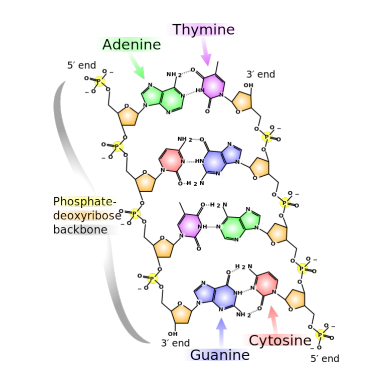
\includegraphics[width=11cm]{chaps/lr/DNA_double_helix}}
	\caption{مارپیچ دوگانه \gls{dna}}
	\label{fig:ch_lr:DNA_double_helix}
\end{figure}



همانند سازی \gls{dna} فرآیند تولید دو مولکول \gls{dna} یکسان از مولکول \gls{dna} اصلی است. وقتی تکثیر شروع می‌شود، دو رشته یک مولکول \gls{dna} از یکدیگر جدا می‌شوند و هر رشته به عنوان الگویی برای ساخت نمونه مشابه خود عمل می‌کند. نوکلئوتید‌ها در هر موقعیت از یک رشته با نوع دیگری از \gls{nucleotid} مبتنی بر قانون پایه جفت شدن، به منظور سنتز همتای این رشته، متصل می‌شود. پس از همانند سازی، مولکول \gls{dna} اصلی به دو مولکول یکسان تبدیل می‌شود (شکل \ref{fig:ch_lr:DNA_replication}) \cite{alberts2002molecular}.

\begin{figure}[!ht]
	\centerline{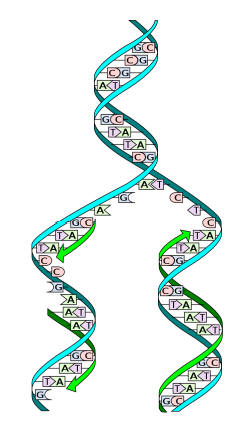
\includegraphics[width=8cm]{chaps/lr/DNA_replication}}
	\caption{همانندسازی \gls{dna}}
	\label{fig:ch_lr:DNA_replication}
\end{figure}





ژن ناحیه‌ای از \gls{dna} است و به عنوان مولکول واحد وراثت شناخته می‌شود. ژن‌های متعددی در ساختار \gls{dna} با عملکرد‌های متفاوت وجود دارد. جهش به تغییر دائمی‌توالی هسته‌ای ژنوم اتلاق می‌شود. جهش‌ها می‌توانند در حین فرآیند تکثیر \gls{dna} و با جفت‌گیری اشتباه در قسمت‌های مختلف \gls{dna} ایجاد می‌شود. انواع مختلفی از جهش‌ها مانند \gls{snm}(\gls{pointmutation})  (شکل \ref{fig:ch_lr:single_nucleotide_mutation}) و  \glspl{singlevariant}  شامل \gls{insertion} ، \gls{deletion}  و \gls{reversion}  (شکل \ref{fig:ch_lr:structural_changes}) وجود دارد. جهش‌های سلولی می‌توانند به بنا بر دلایلی چون مواد شیمیایی، سمیت یا ویروس ایجاد شوند. جهش در یک ژن می‌تواند محصولات آن را تغییر دهد (مانند ایجاد پروتئین متفاوت) یا از عملکرد صحیح ژن جلوگیری کند \cite{alberts2002molecular}.




\begin{figure}[!ht]
	\centerline{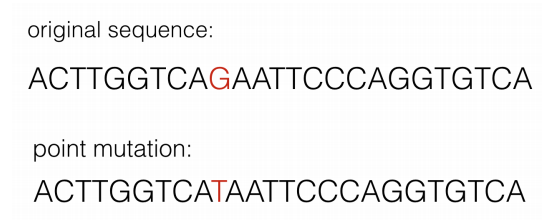
\includegraphics[width=10cm]{chaps/lr/single_nucleotide_mutation}}
	\caption{جهش تک‌نوکلئوتیدی}
	\label{fig:ch_lr:single_nucleotide_mutation}
\end{figure}



\begin{figure}[!ht]
	\centerline{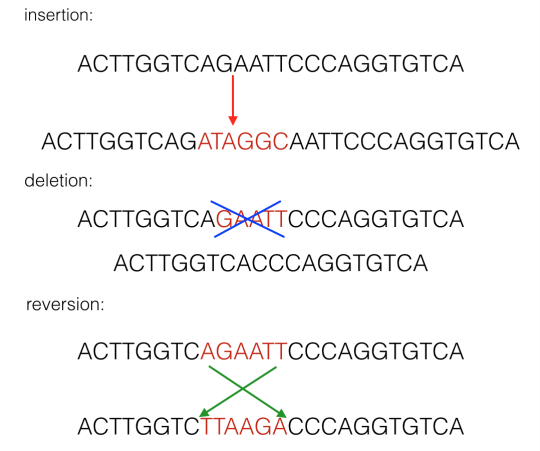
\includegraphics[width=10cm]{chaps/lr/structural_changes}}
	\caption{تغییرات ساختاری}
	\label{fig:ch_lr:structural_changes}
\end{figure}




\section{\gls{tumorevolution}}


جهشی که در هر سلول از بدن اتفاق می‌افتد، به استثنای سلول‌های جنسی (اسپرم و تخمک)، جهش \gls{somatic}  نامیده می-شود \cite{somaticMutation}. تجمع جهش بدنی در طول زندگی یک فرد می‌تواند منجر به رشد کنترل نشده مجموعه‌ای از سلول(تومور) شود \cite{nowell1976clonal} و می‌تواند باعث شکل‌گیری سرطان یا بیماری‌های دیگر شود \cite{somaticMutation}. بدلیل تجمع سلول‌های گوناگون، بیش از یک نوع سلول در تومور وجود خواهد داشت. به گروه‌های سلول با مجموعه‌ای از جهش مشخص، کلون یا جمعیت سلولی تومور گفته می‌شود. کلون‌های موجود در تومور از نظر فیلوژنتیک با هم مرتبط هستند و رابطه آنها را می‌توان با یک درخت فیلوژنتیک نشان داد \cite{birbrair2014type}. درخت فیلوژنتیک رابطه تکاملی بین کلون و ترتیب وقوع هر جهش را نشان می‌دهد. به عنوان مثال، شکل\ref{fig:ch_lr:tumor_phylogenetic_tree} :

\begin{itemize}
	\item یک درخت فیلوژنتیک از یک تومور با چهار کلون با برچسب $0$ تا $3$ را نشان می‌دهد.
	\item جهش جدیدی را نشان می‌دهد که در هر کلون در طول تکامل این تومور رخ داده است.
\end{itemize}

 همچنین هر کلون جهشی را در مسیر از کلون بالایی به سمت خود به ارث می‌برد. به عنوان مثال، کلون $0$ جهش‌های
  $m_0$ و	 $m_1$ دارد. کلون $1$ دارای جهش $m_0$، $m_2$، $m_3$ و $m_4$ است.
 
\begin{figure}[!ht]
	\centerline{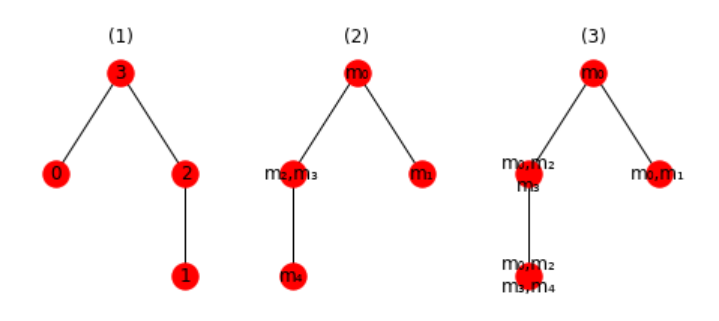
\includegraphics[width=13cm]{chaps/lr/tumor_phylogenetic_tree}}
	\caption{درخت فیلوژنیک تومور}
	\label{fig:ch_lr:tumor_phylogenetic_tree}
\end{figure}


\section{تکنولوژی‌های توالی‌یابی و \gls{variantallelefrequency}}




تعیین توالی \gls{dna} روشی برای تشخیص ترتیب دقیق \glspl{nucleotid} در یک رشته \gls{dna} است. روش \gls{nextgenerationsequencing}  از تعدادی فناوری مدرن توالی تشکیل شده است که امکان تعیین هزینه و زمان توالی‌یابی را به طور موثر فراهم می-کند. با استفاده از نمونه بیولوژیکی به عنوان ورودی این تکنولوژی‌ها، توالی‌های کوتاه نوکلئوتیدی تولید می‌شود (که به آن \gls{read}  گفته می‌شود). سپس خوانش با استفاده از الگوریتم \gls{alignment}  متنوعی مانند الگوریتم تبدیل \lr{Burrows-Wheeler} با ژنوم مرجع تراز می‌شوند. پس از ترازبندی، می‌توان با جمع‌آوری \glspl{overlappingread}،  توالی \gls{consensus}  ایجاد کرد (شکل \ref{fig:ch_lr:alignment_reading}). در موقعیتی از توالی اجماع به دلیل همپوشانی خوانش ها، ممکن است بیش از یک نوع خوانش از \gls{nucleotid} تراز شده وجود داشته باشد (تعداد کل قرائت مرتبط با یک نوع جهش، را \gls{readcoverage}  نامیده می‌شود). \gls{nucleotid} موجود در این موقعیت به عنوان رایج‌ترین \gls{nucleotid} تراز شده، مشخص می‌شود. به عنوان مثال، در شکل \ref{fig:ch_lr:alignment_reading}، سه آدنین (A)، یک گوانین (G) و یک تیمین (T)  در موقعیت سوم توالی اجماع تراز می‌شوند، سپس \gls{nucleotid} در آن موقعیت به عنوان آدنین (A) تعیین می‌شود. پس از ایجاد توالی اجماع، نوکلئوتیدهای موجود در آن توالی، که متفاوت از ژنوم مرجع هستند، شناسایی شده و به عنوان \gls{somaticsnv}  شناخته می‌شود. با استفاده از نمونه‌های متعدد استخراج شده از یک نمونه تومور، ما می‌توانیم تغییرات بدنی تک نوکلئوتیدی را در هر نمونه با فناوری تعیین توالی‌یابی تشخیص دهیم. نسبت تعداد سلول‌های موجود در یک نمونه حاوی تغییرات بدنی تک نوکلئوتیدی به کل سلول‌ها، فراوانی تغییرات آلل یک تغییر بدنی تک نوکلئوتیدی در این نمونه نامیده می‌شود. مقادیر فراوانی تغییرات آلل برای هر تغییر بدنی تک نوکلئوتیدی  در هر نمونه تومور قابل محاسبه است. ابزارهای زیادی برای بازسازی درخت فیلوژنتیک تومور از مقادیر فراوانی تغییرات آلل تومور به عنوان ورودی الگوریتم استفاده می‌کنند.



\begin{figure}[!ht]
	\centerline{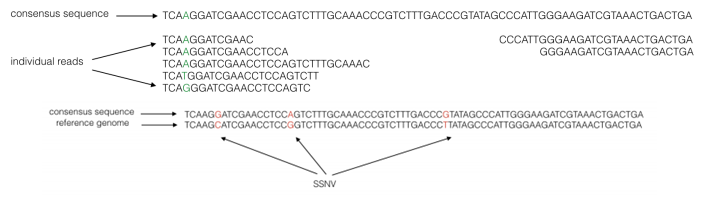
\includegraphics[width=\textwidth]{chaps/lr/alignment_reading}}
	\caption{تشخیص تغییر بدنی تک‌نوکلئوتیدی از طریق خوانش هم‌ترازی}
	\label{fig:ch_lr:alignment_reading}
\end{figure}



\section{ناهمگنی ژنومی تومور}

سرطان بیماری‌ای است که بدلیل ایجاد ناهنجاری‌های اساسی در فرآیند‌های بنیادی سلول مانند \gls{replication}، \gls{differentiation}  و \gls{death} سلول  ایجاد می‌شود \cite{hanahan2011hallmarks}. این ناهنجاری منجر به رشد کنترل نشده تومور و به‌کارگیری بافت غیرسرطانی برای حمایت از این رشد می‌شود. علت اصلی این تغییرات جهش است. جهش یک اصطلاح گسترده است که چندین دسته از تغییرات ژنتیکی را پوشش می‌دهد. هنگام حاملگی، یک جنین دارای یک ژنوم خاص و منحصر به فرد است. این ژنوم که به \gls{germlinegenome} معروف است، می‌تواند با ژنوم انسانی مرجع مقایسه شود. ژنوم انسانی مرجع یک نمونه از ژنوم انسان است و از \gls{dna} چند نفر تشکیل شده است. تفاوت بین ژنوم جوانه‌زنی و ژنوم مرجع به عنوان جهش ژنوم جوانه زنی شناخته می-شود. جهش‌های جوانه زنی می‌توانند مسئول افزایش خطر ابتلا به سرطان باشند \cite{stewart2017world}، اما بندرت خود مسئول مستقیم توسعه تومور هستند. 




معمولاً تومورها در اثر جهش‌های اکتساب شده پس از لقاح، که معروف به جهش‌های بدنی هستند، ایجاد می‌شوند. جهش-های بدنی نتیجه اشتباهات در تکثیر \gls{dna} \cite{behjati2014genome}، قرار گرفتن در معرض جهش‌های با منشأ داخلی یا خارجی یا وارد‌شدن توالی‌های \gls{dna} با منشأ بیرونی بدلیل قرار گرفتن در معرض ویروس است \cite{talbot2004viruses}. غالباً در سرطان، جهش‌های بدنی باعث ایجاد اختلال در روند تکثیر \gls{dna} یا ترمیم آن می‌شوند و حتی جهش‌های بدنی بیشتری ایجاد می‌کنند \cite{stratton2009cancer}. نظریه کلونی بودن سرطان \cite{nowell1976clonal} سرطان را به عنوان یک تک سلولی با منشأ غیرجنسی در نظر می‌گیرد که در اثر تولید مثل فراوان، یک توده متشکل از کلون‌های سلولی گوناگون را ایجاد می‌کند. در این مدل سلولهای توموری با یکدیگر در رقابت هستند و جهش‌های بدنی که مزیت رشد را ایجاد می‌کنند در جمعیت سلول‌های توموری از نسبت بیشتری برخوردار خواهند بود. جهش‌های بدنی که باعث رشد تومور شده و از سلولی به سلولی دیگر منتقل می‌شوند به عنوان \glspl{drivermutation} شناخته می‌شوند. اولین سلولی که دارای جهش راننده بوده و آن را به جهش‌های بعدی منتقل می‌کند به عنوان سلول بنیانگذار شناخته می‌شود. همه فرزندان این سلول بنیانگذار، جهش راننده و هر جهش دیگری را که سلول بنیانگذار قبل از به دست آوردن جهش راننده بدست آورده است، دارند. این جهش‌های دیگر، که مزیتی برای رشد و گسترش تنوع توموری ندارند، به عنوان \glspl{passengermutation} شناخته می‌شوند. شایان ذکر است که تعریف جهش راننده و مسافر به زمینه ژنتیکی و محیطی بستگی دارد. به عنوان مثال، شیمی درمانی \gls{cytotoxic}  (سیتوتوکسیک) می‌تواند باعث تغییر جهش از مسافر به جهش راننده شود و عامل اصلی مقاومت در برابر درمان باشد. همچنین جهش ها را می‌توان بر اساس نوع تغییری که در \gls{dna} ایجاد می‌شود، به طبقات متمایز تقسیم کرد. \gls{snv} جهش‌هایی هستند که یک پایه در ژنوم را به پایه دیگری تغییر می‌دهند. \gls{indel}  درج یا حذف یک بخش \gls{dna} است که می‌تواند کوتاه یا طولانی باشد. از ایندل کوتاه و تغییرات تک نوکلئوتیدی در مجموع به عنوان \glspl{ssm}  یاد می‌شود. در همه قسمت‌های یک ژنوم، از جمله کل کروموزوم‌ها، قابلیت حذف یا کپی شدن قسمتی از ژنوم وجود دارد. تغییرات شماره کپی  به جهشی اتلاق می‌شود که منجر به حذف یا کپی شدن قسمتی از ژنوم می‌شود. \gls{cna} نوعی \gls{singlevariant} هستند که شامل وارونگی (وقتی قسمت بزرگی از ژنوم معکوس شده باشد) و انتقال متعادل (جایی که دو بخش ژنومی مکان‌‌های خود را با یکدیگر تعویض می‌کنند) می‌باشند\cite{stratton2009cancer}. این گونه‌های مختلف جهش مستقل از یکدیگر نیستند و می‌توانند در رابطه با یکدیگر اتفاق بیفتند (به عنوان مثال یک جهش می‌تواند منجر به تقویت یک وارونگی شود). 



تکنیک توالی‌یابی نسل بعدی این امکان را فراهم کرده است تا با صرف هزینه بسیار کم و با استفاده از یک نمونه توموری، توالی‌یابی از \gls{dna} صورت پذیرد و همین امر منجر به تحول گسترده‌ای در زمینه مطالعه تکامل تومور شده زیر امکان نمونه-برداری در تعداد بسیار بالا را از تومور فراهم می‌کند. نمونه‌گیری در حجم بالا این امکان را فراهم آورده است تا ناهمگنی تومور از نقطه منظر ژنتیکی مورد بررسی قرار گیرد و پاسخ به درمان بیماران سرطانی با جزییات بیشتری مورد ارزیابی قرار گیرد.


تقریباً همه نمونه‌های استخراج شده از تومور ترکیبی از سلول ها با ژنوتیپ‌های مختلف را شامل می‌شود. یک نمونه توموری به ندرت فقط شامل بافت سرطانی است زیرا شامل سلول‌های غیر سرطانی از \gls{surroundingstroma}  یا \glspl{Infiltratingimmunecell}  است. مطالعات ژنومیک نشان داده است که حتی در میان سلولهای سرطانی، غالباً زیرجمعیت‌های متعدد سرطانی نیز وجود دارد. به عنوان مثال، در یک مطالعه مهم در سال 2012، گرلینگر و همکارانش \cite{gerlinger2012intratumor} توالی‌یابی ژنوم و تغییرات شماره کپی را از طریق نمونه‌های مکانی مجزا استخراج شده از سرطان کلیه اولیه و نقاط متاستاز ثانویه بدست آورده‌اند. با بررسی  این نمونه‌های متعدد، مشخص شد که یک ناهمگنی ژنتیکی قابل توجهی در تومور وجود دارد. تعداد بسیار زیادی از جهش‌های شناسایی شده در همه سلول‌های توموری مشاهده نشدند و این بدان معناست که این جهش‌ها بیش از آن‌که یک ناحیه کلونی باشند، به صورت یک ناحیه زیر کلونی بوده‌اند. با استفاده از روش‌های پردازش غیراتوماتیک، تغییرات تک نوکلئوتیدی  ها و تغییرات شماره کپی بر اساس نمونه‌هایی که از آن استخراج شده‌اند، به خوشه‌های مجزا دسته‌بندی شده و یک درخت فیلوژنی به آن‌ها نسبت داده شد. بازسازی درخت فیلوژنیک تومور این امکان را فراهم آورد تا سیر تکاملی تومور با استفاده از شاخه‌های مختلف درخت فیلوژنی شامل جهش‌هایی با عملکرد یکسان از سه ژن متفاوت مورد بررسی قرار گیرد. 


در همان سال، یک مطالعه مهم دیگر، "تاریخچه زندگی 21 سرطان پستان`` \cite{nik2012life}، حضور \lr{ITH} را نیز نشان داد. در این مطالعه آنها توالی‌یابی کامل ژنوم را در عمق متوسط \lr{188X} بر روی تومور پستان \lr{PD4120a} انجام دادند. این عمق اجازه می‌دهد تا جمعیت‌های شیوع تا 5٪ کم باشد. آنها مشاهده کردند که تغییرات تک نوکلئوتیدی‌ها در تعداد کمی از خوشه‌های مجزا مشاهده می‌شوند که با توجه به کسر نوع آلل (\lr{VAF}) آنها مشاهده می‌شود، نسبت خواندن ها در یک مکان متفاوت شامل آلل نوع. علاوه بر این، آنها توانستند نشان دهند که برخی از این خوشه‌های مجزا را نمی‌توان با جهش‌های موجود در تمام جمعیت‌های سرطانی توضیح داد، که این نشان دهنده حضور تغییرات تک نوکلئوتیدی‌های تحت کلونال است. در همان زمان، آنها دریافتند که بسیاری از جهش‌ها در تمام سلول‌های سرطانی موجود در نمونه وجود دارد، که نشان می‌دهد جد مشترک اخیر نسبتاً دیر در زمان تکامل رشد کرده است. مشاهده اینکه جهش‌های زیر کلونال به جای توزیع یکنواخت یا مطابق قانون قدرت در خوشه‌های متمایز پیدا شده است، شواهدی را نشان می‌دهد که این جهش‌های زیرکلونالی بیش از آنکه ناشی از تکامل خنثی یا مصنوعات فنی باشد، در زیرمجموعه‌های متمایز ناشی از فشارهای انتخابی یافت می‌شود. نویسندگان همچنین با تأیید اینکه جهش‌های زیر کلونال محدود به تغییرات تک نوکلئوتیدی  نیستند، توانستند حضور تغییرات شماره کپی‌های کلونال و زیرکلونال را تأیید کنند. نویسندگان یک الگوریتم خوشه‌بندی غیر پارامتریک (یک مدل مخلوط فرآیند دیریشله (\lr{DPMM})) را با استدلال قابل توجه دستی برای استنباط فیلوژنی شاخه‌ای از چهار زیر جمعیت سرطانی در آن نمونه منفرد تومور ترکیب کردند. درک معماری ژنتیکی این زیرجمعیت‌ها می‌تواند به مطالعه زیست شناسی سرطان کمک کند و نشان داده شده است که در پیش‌بینی بقا در بسیاری از انواع سرطان مفید است \cite{andor2016pan}. به عنوان مثال، زیرجمعیت‌های مختلف، که توسط مجموعه جهش‌های جسمی حمل شده تعریف می‌شوند، توانایی‌های مختلفی در مقاومت در برابر درمان و متاستاز دارند. برای انجام این کار، باید از یک یا تعداد کمی از نمونه‌های تومور فله، ژنوتیپ‌های موجود در نمونه را شناسایی کرد. این مسئله، تحت عنوان بازسازی ساب کلونال، موضوع اصلی این پایان‌نامه است. مطالعات پیشگام که نشان داد \lr{ITH} برای انجام این بازسازی به استدلال دستی قابل توجهی نیاز دارد. استدلال دستی کند، مستعد خطا است و به تخصص قابل توجهی نیاز دارد. مزایای بازسازی کاملاً خودکار بدیهی است. این بخش پیش زمینه مشکل بازسازی زیر کلونال، چگونگی پرداختن به آن برای انواع مختلف جهش، خصوصیات اصلی الگوریتم‌های بازسازی زیر کلونال و خلاصه‌ای از کارهای موجود در این زمینه را توصیف می‌کند.


\section{بازسازی زیر کلونال }

بازسازی ساب کلونال سعی دارد ژنوتیپ‌های موجود در تومور را از تعداد کمی از نمونه‌های توالی \gls{dna} از آن تومور استنباط کند. تعداد ژنوتیپ‌های موجود در تومور از قبل مشخص نیست. این ژنوتیپ‌های زیر کلونال به طور معمول با جهش‌هایی که در مقایسه با ژنوم خط جوانه‌ای دارند، توصیف می‌شوند. ژنوم جوانه‌زنی علاوه بر نمونه(های) تومور، با تعیین توالی یک نمونه غیرسرطانی تعیین می‌شود. در حال حاضر در هنگام تعریف این جمعیت از دو نوع جهش به طور معمول استفاده می‌شود: جهش‌های ساده بدنی‌های متشکل از تعویض‌ها و درج / حذف کوچک (ایندل) و \gls{cna} حاصل از تغییرات ساختاری بزرگتر. مشاهده انواع جهش‌های دیگر، مانند مجموعه گسترده‌ای از \lr{SV}‌ها که شامل بازآرایی هستند، مشاهده آنها دشوارتر است و روش‌های شناسایی آنها در مراحل اولیه رشد است.


به طور متوسط، حتی در شرایط ایده آل، هر سلول در هر بخش یک جهش پیدا می‌کند \cite{behjati2014genome}، به همین ترتیب، بیشتر سلول‌های تومور ژنوتیپ منحصر به فردی خواهند داشت. بنابراین، به طور دقیق، اکثر سلولهای تومور می‌توانند به طور بالقوه نمایانگر زیرجمعیت منحصر به فرد خود باشند. با این حال، به طور عملی، جهش‌هایی که مختص سلول‌های منفرد است یا فقط تعداد کمی از سلول‌ها آنها را به اشتراک می‌گذارد، در حین فراخوانی نوع شناسایی نمی‌شوند. تماس متغیر در بخش 2.5.3 بیشتر مورد بحث قرار گرفته است. بعلاوه، سلول‌هایی که بخش عمده‌ای از جهش‌های خود را به اشتراک می‌گذارند، خصوصاً جهش‌های راننده، صفات مشابهی دارند. به همین ترتیب، من قرارداد گسترده‌ای را اتخاذ کرده و یک زیر جمعیت را به عنوان تمام سلول‌هایی که دارای زیر مجموعه یکسان جهش‌های بدنی در هنگام فراخوانی نوع هستند، تعریف می‌کنم.


یک گام مهم در بازسازی ساب کلونال محاسبه شیوع سلولی تبارهای زیر کلونال و سپس، در نهایت، زیرجمعیت‌های سرطانی است. شیوع سلولی یک زیرجمعیت، نسبت سلول‌های نمونه توالی شده متعلق به آن است. غالباً، شیوع سلولی با تقسیم بر خلوص نمونه، یعنی نسبت سلولهای سرطانی در نمونه، به بخش سلولهای سرطانی، نسبت سلولهای سرطانی، تبدیل می‌شود. هر سلول دقیقاً به یک زیرمجموعه تعلق دارد، بنابراین این شیوع باید در یک جمع باشد. به طور کلی، سلول‌های غیر سرطانی در یک زیرمجموعه واحد قرار می‌گیرند. با این حال، از آنجا که جهش‌ها اغلب در زیرجمعیت‌های متعدد وجود دارند، شیوع سلولی بسیاری از زیرجمعیت‌ها را نمی‌توان مستقیماً از جهش‌های آن استنباط کرد. برای پرداختن به این موضوع، ما یک نسب زیر کلونال برای یک جهش به عنوان مجموعه زیرجمعیت‌هایی که در آن وجود دارد، تعریف می‌کنیم. به طور رسمی، دودمان‌های زیر کلونال از زیر جمعیت بنیانگذار تشکیل می‌شود (جایی که جهش برای اولین بار ظاهر می‌شود) و همه زیرجمعیت‌های بعدی آن (که وراثت جهش) علاوه بر جهش‌های خاص خود، این زیرمجموعه‌های فرزندی حاوی تمام جهش‌های موجود در نژاد تعریف کننده زیر جمعیت هستند (به جز در صورت حذف محل منبع جهش، برای جزئیات بیشتر به فصل 3 مراجعه کنید). نسب مربوط به یک زیر درخت (یا کلاد) از درخت کلون تومور است. شیوع سلولی یک تبار مجموع شیوع سلولی زیرجمعیت‌هایی است که متعلق به آن تبار هستند. از آنجا که سلول‌ها می‌توانند در چندین نژاد زیرکلونال وجود داشته باشند، شیوع نسب در یک جمع نیست.



شکل \ref{fig:ch_lr:tumor_clone_tree} تصویری از یک درخت کلون نمونه را ارائه می‌دهد. گره‌های موجود در درخت، همانطور که در بالا تعریف شد، نشان دهنده زیر جمعیت است. فلش‌ها از جمعیت والدین به سمت فرزندانشان هدایت می‌شوند. دودمانهای زیر کلونال به صورت مستطیل نشان داده می‌شوند و با توجه به زیرمجموعه بنیادی آنها که در ریشه تیغه یافت می‌شوند، رنگی هستند.


\begin{figure}[!ht]
	\centerline{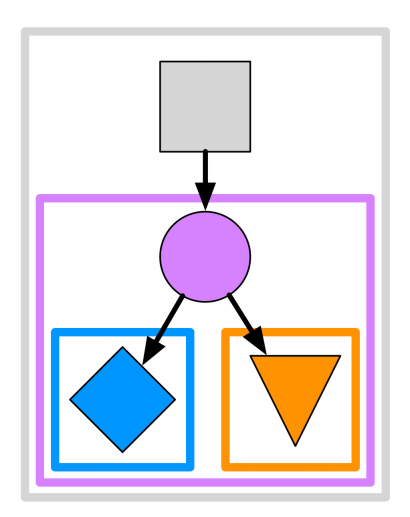
\includegraphics[width=7cm]{chaps/lr/tumor_clone_tree}}
	\caption{درخت کلون تومور}
	\label{fig:ch_lr:tumor_clone_tree}
\end{figure}




\section{تغییرات تعداد کپی}

بیشتر ژنوم انسان دیپلوئید است، به این معنی که دو نسخه از توالی \gls{dna} ما در سلول‌های ما وجود دارد، یکی از پدر و دیگری از مادر. تغییرات شماره کپی این تغییر را می‌دهند، یا با تغییر در تعداد نسخه‌ها (مثلاً از طریق تکثیر کل ژنوم)، نسبت کپی‌های مادر به پدر (مثلاً از دست دادن خنثی هتروزیگوزیته در تعداد کپی‌ها، جایی که برای همان منطقه یک ژنوم والدین تکثیر می‌شود و دیگری حذف شده است) یا هر دو (به عنوان مثال کپی کروموزوم مادر). بیشتر این تغییرات (به استثنای تکثیر کل ژنوم) دامنه محدودی از ژنوم را تحت تأثیر قرار می‌دهد، اما می‌تواند از تأثیر یک ژن تا یک کروموزوم کامل باشد. این بخش از ژنوم تغییر یافته به عنوان یک بخش شناخته می‌شود.


تغییرات شماره کپی می‌توانند تعداد کپی کل یک بخش و / یا تعداد نسبی نسبی دو کروموزوم والدین را تغییر دهند. هر یک از این تغییرات توسط توالی‌یابی ژنومی هسته قابل تشخیص است. تغییر در تعداد کپی کل یک بخش را می‌توان تشخیص داد زیرا نسبت خواندن آن نقشه به آن بخش بین خط جوانه زنی و نمونه تومور متفاوت خواهد بود. بخش از یک قطعه نسبت ورود خوانده شده است که به یک قطعه در یک نمونه غیر سرطانی ترسیم شده است به نسبت خوانده شده که به یک بخش در یک نمونه سرطانی ترسیم شده است. از نسبت نسبت‌ها برای محاسبه این واقعیت استفاده می‌شود که تعداد کل قرائت‌ها اغلب بین توالی‌یابی سرطانی و غیرسرطانی متفاوت است، در مناطق مختلف ژنوم عمق خواندن بیشتر یا پایین‌تر ناشی از محتوای \lr{GC} یا نقشه برداری وجود دارد و تردستی یک تومور با بافت طبیعی متفاوت است. تکرر یک ژنوم، میانگین تعداد کپی از هر کروموزوم است که برای طول کروموزوم نرمال می‌شود.


با تغییر در کسر آلل می‌توان عدم تعادل در تعداد نسخه‌های مادری و پدری این بخش را تشخیص داد. در مناطق دیپلوئید ژنوم‌ها، اگر یک بازه بین کپی‌های مادر و پدر متفاوت باشد، موقعیت هتروزیگوت نامیده می‌شود. جهش‌های تک پایه، خط جوانه زنی همچنین به عنوان چند شکلی تک هسته‌ای نامیده می‌شوند. وقتی یک ژنوم توالی‌یابی شود، حدود نیمی از قرائت آن مکان هتروزیگوت حاوی هر یک از بازها خواهد بود، در نتیجه کسر آلل 50 است. این امر تا زمانی که نسبتی برابر با نسخه‌های مادرانه و پدری وجود داشته باشد، صادق خواهد بود. اگر این نسبت تغییر کند، کسر آلل  تمام پولیمورفیسم تک هسته‌ای در بخش آسیب دیده تغییر می‌کند. پولیمورفیسم تک هسته‌ای هتروزیگوت به طور متوسط هر 1500 باز \cite{chen2012personal} رخ می‌دهد و بنابراین برای بخشهای طولانی بسیاری از پولیمورفیسم تک هسته ایی هتروزیگوت تحت تأثیر قرار می‌گیرند. توزیع کسر آلل \lr{S} تمام پولیمورفیسم تک هسته‌ای در بخش، حالت دوگانه‌ای پیدا می‌کند که هر حالت نشان دهنده نسبت نسخه‌های آن بخش از هر والد است.

فراخوانی \lr{CNA} چالش برانگیز است زیرا با مشاهده مستقل هر بخش، مسئله هنوز مشخص نشده است. حتی با فرض اینکه هر بخش فقط توسط یک \lr{CNA} تحت تأثیر قرار گیرد، \lr{CNA} موسوم به سه پارامتر (نسبت سلولهای حاوی \lr{CNA}، تعداد کپی‌های مادر و تعداد کپی‌های پدری) وجود دارد و فقط دو مشاهده برای توضیح وجود دارد (و کسر آلل )

همه روش‌ها با فرض اینکه تعداد کمی از نژادهای زیرکلونال مسئول بیشتر یا تمام تغییرات شماره کپی هستند، این ابهام را برطرف می‌کنند. روشی که توسط الگوریتم باتنبرگ \cite{nik2012life} به کار رفته است، به بیشتر تغییرات شماره کپی وابسته به یک نژاد زیر کلونال منفرد و شایع به نام تبار کلونال متکی است. تحت این روش، شیوع این تبار، همراه با تعداد کپی اصلی و جزئی در تمام تغییرات تعداد کپیکلونال، می‌تواند با یک فرآیند دو مرحله‌ای تخمین زده شود. در گام اول، این روش با فرض شیوع نژاد کلون $f_c$  آغاز می‌شود. شیوع تبار کلونال در بیشتر موارد با خلوص نمونه تومور برابر است. با توجه به شیوع کلونال، هر بخش پس از آن فقط دو متغیر برای توضیح دارد (تعداد کپی بزرگ و جزئی). از آنجا که هر بخش دارای دو مشاهدات است، اکنون مسئله هنوز به درستی تعیین نشده است و بهترین کپی اصلی و مینور متناسب است. سپس، ترکیب کلی مقدار $\Phi_c$  فرض شده با ترکیب مناسب در تمام بخشها تعیین می‌شود. الگوریتم با بهینه سازی این تناسب بهترین مقدار $\Phi_c$  را انتخاب می‌کند. سپس برای هر بخش، شماره کپی اصلی و جزئی با بهینه سازی متناسب بودن قطعه با بهترین مقدار $\Phi_c$   انتخاب می‌شود. این روش فرض می‌کند که تمام تغییرات شماره کپی به نژاد کلونال تعلق دارند، که همیشه درست نیست. در مرحله بعدی، بخشهایی که حاوی تغییرات تعداد کپیتحت کلونال هستند با جستجوی بخشهایی با اطلاعات مناسب ضعیف با استفاده از $\Phi_c$   استنباط شده مشخص می‌شوند. در این بخش‌ها، روش به طور همزمان و مستقل از هر بخش دیگر، عدد $\Phi_i$   و عدد کپی بزرگ و جزئی را استنباط می‌کند.


از آنجا که سه متغیر وجود دارد و تنها دو مشاهده وجود دارد، راه حل‌های بسیاری با تناسب داده برابر وجود دارد که از نظر زیست شناختی برای این تغییرات تعداد کپی زیر کلونال قابل قبول است. این ابهام با انتخاب راه حلی که نزدیکترین شماره به شماره نسخه طبیعی است برطرف می‌شود، اما تعدادی از موارد متداول وجود دارد که این ابتکار عمل ناموفق است. سپس این روش‌ها انتساب تغییرات تعداد کپی زیرکلونال به دودمان و تمام استنباط‌های فیلوژنتیک را برای روش‌های پایین دست رها می‌کنند.


رویکرد عمده دیگر این است که فرض کنیم همه تغییرات شماره کپی از تعداد کمی تبار ساب کلونال به وجود می‌آیند. الگوریتم‌هایی که از این روش استفاده می‌کنند به طور مشترک شیوع این نژادها و تعداد کپی بزرگ و جزئی را برای هر بخش استنتاج می‌کنند (به عنوان مثال \lr{THetA}\cite{zhu2011metabolic, vander2009understanding} و \lr{TITAN} ).  تعداد دودمانهای زیر کلونال معمولاً با استفاده از احتمال جریمه شده‌ای مانند معیار اطلاعات بیزی (\lr{BIC}) یا انواع \lr{BIC} تعیین می‌شود (به عنوان مثال \lr{THetA} از \lr{BIC} اصلاح شده با پارامتر مقیاس گذاری استفاده می‌کند \cite{zhu2011metabolic}). بنابراین این روش‌ها هم تغییرات شماره کپیرا فراخوانی می‌کنند و هم آنها را به دودمان‌های زیرکلونال اختصاص می‌دهند. هیچ روش موجود این دودمان‌ها را در یک درخت فیلوژنتیک قرار نمی‌دهد



\section{جهش‌های ساده بدنی }

جهش‌های ساده بدنی جهش‌های کوچکی هستند که می‌توانند مستقیماً از طریق توالی‌یابی و نسبت کروموزوم‌های موجود در نمونه حاوی آنها از تعداد قرائت‌های حاوی جهش و تعداد کل خوانده‌ها در آن مکان، مشاهده شوند. نسبت قرائت حاوی جهش به کل قرائت به عنوان \lr{VAF} جهش شناخته می‌شود. جهش‌های ساده بدنی‌ها معمولاً با بررسی مشترک ترازها و یک نمونه غیر‌سرطانی خوانده می‌شوند. این استنباط مشترک برای جداسازی انواع بدنی و ژرمینال مورد نیاز است.

این فرایند به دلیل انواع مختلف خطاها و تعصبات که در داده‌های \lr{NGS} وجود دارد، دشوار می‌شود\cite{friedl2010plasticity}. یک مشکل اساسی در تشخیص جهش‌های ساده بدنی این است که به نظر می‌رسد خطاهای توالی جهش‌های ساده بدنی شیوع کمی دارند. به طور خاص، در  \lr{Illumina Hiseq2000}  که به طور گسترده استفاده می‌شود، از هر 1000 پایه یکی از آنها دارای یک خطا است (به طور معمول یک تعویض) \cite{sabeh2009protease}. به همین ترتیب، در طول سه میلیارد پایه ژنوم انسانی، یک احتمال غیر قابل اغماض وجود دارد که در بعضی موقعیت‌ها، چندین بار خواندن دقیقاً شامل خطای توالی دقیقاً در همان موقعیت‌ها است. به نظر می‌رسد این خطاها شیوع کم جهش‌های ساده بدنی دارند. تمایز بین این خطاها و شیوع کم واقعی جهش‌های ساده بدنی‌ها شامل یک معامله بین حساسیت و ویژگی و در حالت ایده آل، یک مدل نویز بسیار دقیق است. حل این مشکل امتداد طبیعی کار گسترده‌ای است که در زمینه فراخوانی جهش‌های جوانه‌زنی انجام شده است و الگوریتم‌های زیادی برای انجام این کار وجود دارد (به عنوان مثال \cite{friedl2010plasticity, demicheli2008effects} )


\section{\gls{allelecdropout}}

اگرچه روش‌های تعیین توالی با بازدهی بالا \cite{hugo2007epithelial} ارزان هستند، اما تحت تاثیر مقدار بایاس هستند و مارکرهای ژنتیکی‌ای تولید می‌کنند که تقریباً به طور تصادفی در کل ژنوم تقسیم می‌شوند. این روشها با موفقیت در \gls{mapping} صفات \cite{nowell1976clonal, greaves2012clonal}، ساخت مپ پیوندی \cite{sakr1993frequency, fearon1990genetic}،  اسکن انتخاب  \cite{dentro2018portraits, waclaw2015spatial}،  و برآورد تنوع ژنتیکی \cite{de2006clonal} استفاده شده است. یکی از این روش‌ها، تعیین ژنوتیپ براساس توالی \cite{anderson2011genetic} (\lr{GBS}) است. در \lr{GBS}، هدف توالی‌یابی فقط با اتصال آداپتورهای توالی به محل‌های برش آنزیم محدود کننده، به کمتر از $5\%$ از ژنوم کاهش می‌یابد (شکل زیر).  قرائت \lr{GBS} همچنین می‌تواند به صورت کانکت‌های کوتاه مونتاژ شود، که بدون نیاز به توالی ژنوم فراخوانی یک نوع تغییر تک هسته‌ای (تغییرات تک نوکلئوتیدی ) را امکان پذیر می‌کند \cite{hanahan2000hallmarks}. از این رو، \lr{GBS} یک روش محبوب در سیستم‌های غیر مدلی است که به طور معمول فاقد منابعی مانند مجموعه ژنوم و ریزآرایه‌ها است.

بر خلاف توالی‌یابی کل ژنوم \lr{(WGS)}، \lr{GBS} مستعد ابتلا به خطاهای مختلف تماس به دلیل محدودیت چندشکلی‌های سایت  است (کاهش آللیک). کاهش آللیک در \lr{GBS} می‌تواند برنامه‌هایی را که به فراخوانی دقیق تغییرات نادر، از جمله تخمین طیف فرکانس سایت در ژنتیک جمعیت متکی هستند، را دچار اختلال کند. یک رویکرد آماری سیستماتیک برای تشخیص کاهش آللیک در داده‌های توالی \lr{GBS}، اجرا شده و  در بسته نرم افزاری منبع باز \lr{GBStools} وجود دارد.  این روش مبتنی بر این واقعیت است که کاهش آللیک متناسب با تعداد آللهای سایت محدود کننده بدون برش که در آنجا حمل می‌کند، میزان خوانش نمونه را در یک سایت خاص کاهش می‌دهد. بنابراین \lr{GBStools} پوشش هر نمونه را در یک سایت خاص به عنوان یک متغیر تصادفی پواسون مورد استفاده قرار می‌دهد که از توزیع با میانگین \lr{$\lambda$} (آللیک‌های بدون برش صفر)، توزیع با میانگین ½\lr{$\lambda$} (یک آللیک بدون برش)، یا با میانگین صفر (دو آللیک بدون برش). \lr{GBStools} حداکثر احتمال پارامتر \lr{$\lambda$} را با استفاده از تعداد واقعی آللیک‌های بدون برش در هر نمونه که به عنوان متغیرهای نهفته (مشاهده نشده) در نظر رفته می‌شود و از طریق  حداکثر رساندن  مقدار چشم انتظاری \lr{(EM)}، محاسبه می‌کند . از مقادیر مورد انتظار این متغیرهای نهفته می‌توان برای تخمین اینکه کدام نمونه ها یک آللیک بدون برش دارند استفاده کرد. به طور همزمان، \lr{GBStools} فرکانس سایت آلل‌های \lr{SNP} مرجع قابل مشاهده و جایگزین، \lr{$\varphi_1$} و  \lr{$\varphi_2$}  ، و آللیک بدون برش، \lr{$\varphi_3$} ، که در آن  \lr{$\varphi_1$+$\varphi_2$+$\varphi_3$=1}   برآورد می‌کند و در نهایت، آزمون نسبت احتمال با مقایسه فرضیه صفر  \lr{$\varphi_3$ = 0} با فرضیه \lr{$\varphi_3$> 0} جایگزین می‌کند. \lr{GBStools}  در اجرای فعلی خود نمی تواند ژنوتیپ‌های واقعی پنهان شده توسط کاهش آللیک را استنباط کند، اما می‌توان با فیلتر کردن سایت‌هایی که نسبت احتمال آنها زیاد است خطاها را حذف کند.

\begin{figure}[!ht]
	\centerline{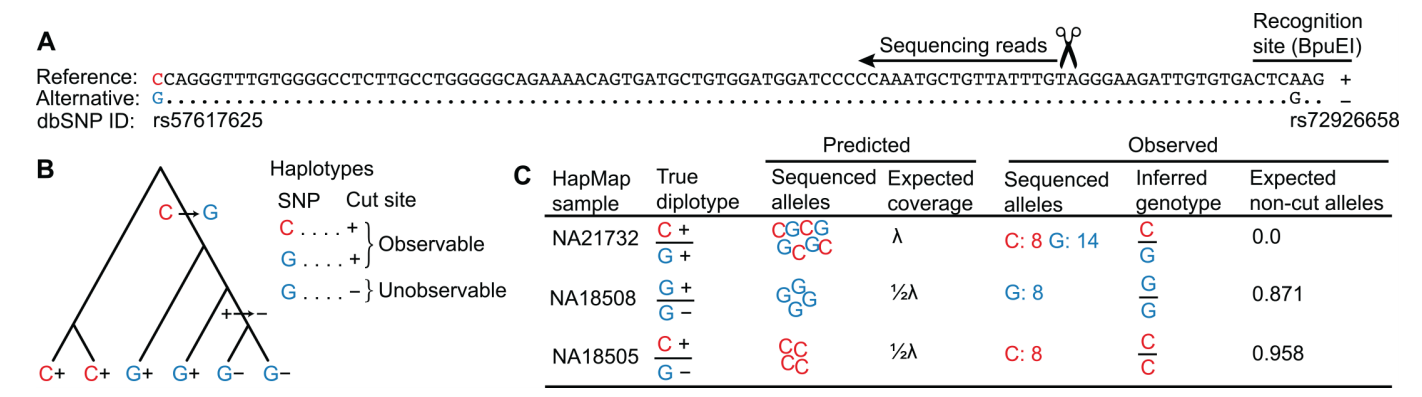
\includegraphics[width=\textwidth]{chaps/lr/mtsd}}
	\caption{نمایی از تطابق ژنتیکی}
	\label{fig:ch_lr:mtsd}
\end{figure}

در شکل بالا، آلل \lr{BpuEI} بدون برش ناشی از \lr{SNP rs72926658} با برچسب "-`` و آلل برش با "+`` برچسب گذاری شده است. آلل "-`` در هاپلوتیپ با آلل \lr{G} مشتق شده بوجود آمده و باعث شده تا برخی از آلل‌های \lr{G} توسط \lr{GBS} قابل مشاهده نباشند. نمونه‌های نشان داده شده دارای سه دیپلوتیپ هتروزیگوت است. نتایج توالی با پیش‌بینی‌ها مطابقت داشت و نمونه \lr{NA18505} به اشتباه هموزیگوت نامیده می‌شد، اما انتظار می‌رود تعداد آلل‌های کاهشی محاسبه‌شده توسط \lr{GBStools (0.958)} با تعداد واقعی (1) مطابقت داشته باشد، و آن را به عنوان یک تماس اشتباه احتمالی مشخص کند.

\section{مقدمه‌ای بر مدل‌سازی احتمالی }

وظیفه اصلی یادگیری ماشین، یادگیری از داده‌ها است، کاری که به عنوان استنباط شناخته می‌شود. برای یادگیری از داده‌ها، باید فرضیاتی را مطرح کرد. توصیف رسمی فرضیات صورت گرفته به عنوان یک مدل ذکر می‌شود. یک مدل احتمالی مفروضات ارائه شده را تعریف می‌کند که اطلاعات آموخته شده را با استفاده از متغیرهای تصادفی و توزیع‌های احتمال به داده‌های مشاهده شده پیوند می‌دهد. توزیع‌های احتمال توابع ریاضی هستند که یک رویداد را ورودی می‌کنند و احتمال آن واقعه را بیرون می‌آورند. توزیع احتمال می‌تواند تابعی بیش از واقعه باشد و این متغیرهای اضافی به عنوان پارامترهای توزیع شناخته می‌شوند\cite{hanahan2000hallmarks}. 
رویکرد بیزی در یادگیری ماشین شامل استنباط احتمالی مقادیر پارامترهای منوط به مشاهدات است \cite{hanahan2011hallmarks}. چهار مولفه دارد:

\begin{itemize}
	\item 	احتمال: احتمال مشاهده داده‌ها است، مشروط به تنظیم پارامتر \lr{ P(data | parameters)} 
	\item 	پارامترهای احتمال
	\item	پارامترهای قبلی 
	\item داده‌های مشاهده شده
\end{itemize}
پارامترها خود مجموعه‌ای از متغیرهای تصادفی هستند که از توزیع قبلی (\lr{P} (پارامترها)) گرفته شده اند، که باورهای ما را در مورد احتمال حالت‌های مختلف پارامتر در غیاب مشاهده مشاهده می‌کند. این اصطلاحات با استفاده از قانون بیز با هم ترکیب می‌شوند:
\begin{itemize}
	\item \lr{P(parameters|data) = P(data|parameters) $*$ P(parameters) $/$ P(data)}
	\item \lr{Posterior $\propto$ likelihood  $*$  prior}
\end{itemize}
پس زمینه توزیع پارامترهای مشروط به مشاهده داده‌ها است و خروجی اصلی استنتاج بیزی است. از توزیع پسین می‌توان برای انجام کارهایی مانند پیش‌بینی مشاهدات آینده استفاده کرد.


\subsection{\gls{markovchainmontecarlo}}

برای انجام استنتاج \gls{bayesian}، ما اغلب می‌خواهیم در توزیع پسین ادغام شده، پیش‌بینی کنیم یا خلاصه‌هایی پیدا کنیم، به عنوان مثال میانگین پارامتر پسین. به طور کلی، انجام چنین ادغامی (جمع بندی در مورد متغیرهای گسسته) از نظر تحلیلی غیرقابل حل است. با این حال، می‌توان چنین ادغام‌هایی را با استفاده از نمونه‌هایی که از قسمت پسین ترسیم شده‌اند تقریبی داد:
\begin{equation}
	E[f]=\int f(x) p(x) d x \approx 1 / N \sum_{1 . . N} f\left(x_{i}\right)
\end{equation}
که در آن $x_i$  نمونه $i$ از $p(x)$ و $p(x)$  و $f(x)$ به ترتیب توزیع و عملکرد مورد نظر ما است. به ندرت می‌توان مستقیماً از توزیع پسین نمونه برداری کرد. برای تولید موثر نمونه‌ها از توزیع، حتی در ابعاد بالا، می‌توان از تکنیک زنجیره ماکوف مونت کارلو استفاده کرد. زنجیره ماکوف مونت کارلو یک زنجیره مارکوف می‌سازد که در آن توزیع تعادل توزیع پسین است. سپس مقادیر زنجیره می‌تواند به عنوان نمونه از پسین با توجه به همگرایی کافی به توزیع تعادل مورد استفاده قرار گیرد. برای انجام زنجیره ماکوف مونت کارلو، تاز زمانی که بتوان \lr{$p \propto p(x)$ } را محاسبه کرد، نیازی به محاسبه $p(x)$  نیست. این زنجیره ماکوف مونت کارلو را قادر می‌سازد تا از محاسبه ثابت‌های نرمال سازی، که اغلب غیرقابل حل هستند، خودداری کند.
یک زنجیره مارکوف به عنوان یک سری متغیرهای تصادفی تعریف می‌شود که دارای ویژگی استقلال شرطی زیر هستند:
\begin{equation}
	p\left(z^{N+1} \mid z^{1} . . z^{N}\right)=p\left(z^{N+1} \mid z^{N}\right)
\end{equation}
نمونه‌ای از الگوریتم زنجیره ماکوف مونت کارلو الگوریتم \lr{Metropolis-Hastings (MH)} است \cite{hastings1970monte}. الگوریتم \lr{MH}  از حالت دلخواه   $Z^t$ شروع می‌شود. سپس یک حالت پیشنهادی $z$  از توزیع پروپوزال \lr{$q(z | z^t)$} ترسیم می‌شود. این حالت پیشنهادی $z$   با احتمال زیر پذیرفته می‌شود:
\begin{equation}
	\min \left(1, \hat{p}\left(z^{*}\right) q\left(z^{t} \mid z^{*}\right) / \hat{p}\left(z^{t}\right) q\left(z^{*} \mid z^{t}\right)\right)
\end{equation}
می توان نشان داد که الگوریتم MH تعادل دقیق را برآورده می‌کند و از این رو،$p(x)$ توزیع تعادل است \cite{bishop2006pattern}. در حالی که توازن دقیق برای اثبات اینکه در محدوده نمونه‌های بی‌نهایت زنجیره به توزیع مورد نظر همگراست کافی است، اما در عمل فقط تعداد محدودی از نمونه‌ها را می‌توان ترسیم کرد. واضح است که نمونه‌های ابتدای زنجیره، که از یک مکان دلخواه در فضای حالت شروع می‌شوند، بعید است از توزیع تعادل باشد. این نمونه‌ها به عنوان نمونه‌های سوختنی کنار گذاشته می‌شوند. هرچه همگرایی زنجیره مارکوف سریعتر باشد، نمونه‌های کمتری باید کنار گذاشته شوند و می‌توان از تعداد بیشتری برای محاسبه انتظارات استفاده کرد. با بررسی اثری از مقادیر مهم پارامتر یا احتمال همگرایی می‌توان نظارت کرد، اما این امر ممکن است چند حالت را از دست بدهد. متأسفانه دانستن اینکه آیا همگرایی حاصل شده است غیرممکن است، فقط گاهی اوقات می‌توان همگرایی را رد کرد \cite{gelman2011inference}. گذشته از همگرایی، یکی دیگر از خصوصیات اصلی یک زنجیره مارکوف میزان اختلاط زنجیره است. با توجه به n نمونه مستقل از توزیع، واریانس میانگین پارامتر برآورد $ \sigma_n $ است که $\sigma$ انحراف استاندارد توزیع خلفی پارامتر است. نمونه‌های گرفته شده از زنجیره مارکوف مستقل نیستند، زیرا به وضعیت فعلی زنجیره بستگی دارند (یعنی فقط از نظر شرطی مستقل هستند). برای تخمین اندازه نمونه موثر یک زنجیره مارکوف، یعنی تعداد نمونه‌های مستقل با همان خطای استاندارد همان زنجیره، می‌توان از معادله زیر استفاده کرد:
\begin{equation}
	E S S=\frac{n}{1+2 \sum_{0}^{\infty} \rho_{j}}
\end{equation}
حاصل جمع بی نهایت محاسبه \lr{ESS} را می‌توان با استفاده از برآوردگر پریودوگرام کوتاه تطبیقی \lr{Sokal} \cite{sokal1997monte} تخمین زد.


\section{\gls{machinelearning} و \gls{reinforcementlearning}}

آنالیز داده‌های بالینی یک حوزه مهم تحقیقاتی در انفورماتیک، علوم کامپیوتر و پزشکی است که توسط محققان شاغل در دانشگاه‌ها، صنعت و مراکز بالینی انجام می‌شود. یکی از بزرگ‌ترین چالش‌ها در تجزیه و تحلیل داده‌های پزشکی، استخراج و تجزیه و تحلیل داده‌ها از تصاویر است. در چند سال اخیر روش‌های \gls{machinelearning} انقلابی بزرگ در \gls{computervision} به وجود آورده است که راه‌حل‌های جدید و کارآمدی را درمورد خیلی از مسائل و مشکلات موجود در آنالیز تصاویر که مدت زمان طولانی است حل نشده باقی مانده‌اند معرفی می‌کنند. برای اینکه این انقلاب وارد حوزه آنالیز تصاویر پزشکی شود شیوه و روش‌های اختصاصی‌ای باید طراحی شوند تا خاص بودن تصاویر پزشکی را در نظر گیرند. سیستم‌های کامپیوتری هوشمند چندین دهه است که در دنیا جایگاه برجسته‌ای پیدا کرده‌اند. در حال حاضر، به خاطر تکنیک‌های جدید \gls{ai}، قابلیت پردازش کامپیوتری بالا و رشد گسترده تصویربرداری و ذخیره‌سازی دیجیتالی داده، کاربرد \gls{ai} در حال انتقال به حوزه‌های گوناگون می‌باشد. در حوزه پزشکی، سیستم‌های \gls{ai} به منظور آشکارسازی بیماری، پیش‌بینی و به عنوان استراتژی پشتیبان در تصمیم‌گیری بالینی در حال توسعه، کاوش و ارزیابی هستند. در زمینه \gls{breastcancer} از \gls{ai} به منظور آشکارسازی زودهنگام و تفسیر \glspl{mammogram} به منظور بهبود غربالگری سرطان پستان و کاهش تشخیص \gls{falsepositive} استفاده می‌شود و این امکان فراهم شده است تا متخصصانی مانند \glspl{radiologist} بتوانند بر اساس میلیون‌ها تصویر از بیماران قبلی که مشخصات مشابهی دارند، تصمیمات آگاهانه‌ای بگیرند. استفاده از \gls{ai} در شیوه‌های تشخیص \gls{breastcancer} به \gls{imagingmodality} و همچنین تفسیر \gls{pathology} نیز گسترش یافته است. \gls{deeplearning} که زیر شاخه‌ای از \gls{machinelearning} می‌باشد یکی از تکنیک‌های \gls{ai} است که در انواع مختلفی از مسائل کلینیکی و پردازش تصاویر پزشکی شامل \gls{detection}/\gls{recognition}، \gls{segmentation} و \gls{computeraideddiagnosis} به کار گرفته می‌شود.

یادگیری عمیق مجموعه‌ای از الگوریتم‌های ماشین است که قادر به مدل‌سازی الگوها به طور مستقیم از داده‌های خام می-باشد. الگوریتم‌های یادگیری عمیق از مجموعه‌ای از لایه‌های چندگانه با واحدهای پردازنده غیرخطی برای استخراج و تبدیل ویژگی استفاده می‌کنند. هر لایه از خروجی لایه قبل به عنوان ورودی استفاده می‌کند. این مفهوم با بسیاری از روش‌های دیگر یادگیری ماشین که نیاز به استخراج ویژگی دارند متفاوت است. به همین ترتیب این الگوریتم‌ها حتی در مسائلی که دانش بسیار کمی در موردشان وجود دارد، می‌توانند مورد استفاده قرار گیرند. اگرچه در دهه 1990 این الگوریتم‌ها در برخی از مطالعات مورد استفاده قرار گرفته اند، اما در چند سال اخیر شاهد نتایج بسیار چشمگیر این الگوریتم‌ها هستیم. با توجه به وجود داده‌های بیشتر و همچنین قدرت محاسباتی بالا، این روش‌ها در بسیاری از زمینه‌ها توانسته اند به عملکرد انسان یا بهتر از انسان دست یابند\cite{akselrod2017deep}. شبکه‌های عصبی مصنوعی  نوع خاصی از مدل‌های یادگیری عمیق هستند که برای کار با داده‌های از نوع تصویر مناسب هستند.

شبکه‌های عصبی مصنوعی مدل‌هایی هستند که در بسیاری از زمینه‌های تحقیقاتی از جمله یادگیری ماشین کاربرد دارند. یک شبکه عصبی مصنوعی از واحدهای ساده ای به نام \gls{neuron} تشکیل شده است که در یک سیستم پیچیده سازمان یافته اند. هر \gls{neuron} بر اساس ورودی‌های خود، یک خروجی (\gls{activation}‌) را محاسبه می‌کند که می‌تواند فعالیت‌ها یا داده‌های سایر \glspl{neuron} باشد. متداول‌ترین نوع شبکه عصبی،  شبکه عصبی کاملاً متصل \gls{fullyconnectedffnn} است. این شبکه‌ها دارای ورودی (جایی که داده‌ها وارد می‌شوند) و خروجی‌ هستند. به طور معمول، هدف از استفاده از این مدل‌ها حل \gls{regression} یا \gls{classification}، توسط تقریب \gls{activation} خروجی با مقدار هدف، برای هر داده ورودی است. این شبکه‌ها به صورت \glspl{layer} متوالی سازماندهی شده اند که یک \gls{neuron}(واحد) از لایه $k$ تمام \glspl{neuron} \gls{layer} $k-1$ را به عنوان ورودی دریافت می‌کند، ترکیبی خطی از این مقادیر را محاسبه کرده و آن را از طریق تابع غیر خطی عبور می‌دهد

محاسبه خروجی
\gls{neuron} \lr{i}ام \gls{layer} \lr{k}
\begin{equation}
	O_{k, i}=\operatorname{actv}\left(\mathrm{W}_{k, \mathrm{i}} \cdot \mathrm{l}_{\mathrm{k}-1}+b_{k, i}\right)
	\label{eq:ch_lr:activation_out}
\end{equation}

که $O_{k,i}$ واحد $i$ام \gls{layer} $k$  و $l_{k-1}$ بردار تمام \glspl{activation}ی \gls{layer} $k-1$ است. بردار $W_{k,i}$ و عدد $b_{k,i}$ پارامترهای ما هستند که اغلب به آنها \gls{netweight} گفته می‌شود که برای یک وظیفه خاص آموخته می‌شوند. تابع \gls{activation} غیرخطی \lr{actv} می‌تواند اشکال مختلفی  به خود بگیرد. هر مدل با یک لایه پنهان و تعداد مشخصی نورون اگر پارامترهای کافی داشته باشد می‌تواند هر تابع پیوسته ای را با خطا دلخواه تقریب بزند\cite{dhungel2017fully}.


\glspl{convnet}  یک نوع شبکه عصبی مصنوعی هستند که از نورون‌ها، لایه‌ها و وزن‌ها تشکیل شده اند. مطالعه ای که در سال 1968 میلادی صورت گرفت نشان داد که قشر بینایی مغز برای پردازش اطلاعات از تصاویر از الگوی پیچیده ای استفاده می‌نماید\cite{sutherland1968outlines}. نواحی ادراکی که قشر بینایی در آن قرار دارد، همانند فیلترهای محلی بر روی اطلاعات تصویر اعمال می‌شود. سلول‌های ساده‌تر برای تشخیص ویژگی‌های ادراکی سطح پایین‌تر در نواحی ادراکی مانند لبه‌ها کاربرد دارند، همچنین سلول‌های پیچیده قادر به تشخیص ویژگی‌های مهم‌تر و اختصاصی‌تر و در سطوح بالاتر می‌باشند. تشخیص ویژگی‌های اختصاصی‌تر نتیجه و ترکیبی از ویژگی‌های سطح پایین می‌باشد. این عملکرد مغز الهام بخش شبکه‌های عصبی عمیق امروزی می‌باشد. مفهوم شبکه کانولوشن نخستین بار در سال 1980 توسط فکوشیما مطرح گردید\cite{fukushima2007neocognitron}. اما به دلیل نیاز به سخت افزار ها و پردازشگر‌های گرافیکی قوی استفاده از این شبکه ها برای تشخیص تا سال 2012 که به شکل اختصاصی برای تشخیص تصاویر ارایه و معرفی گریدی به تعویق افتاد\cite{lecun2015deep}.

\begin{figure}[!ht]
	\centerline{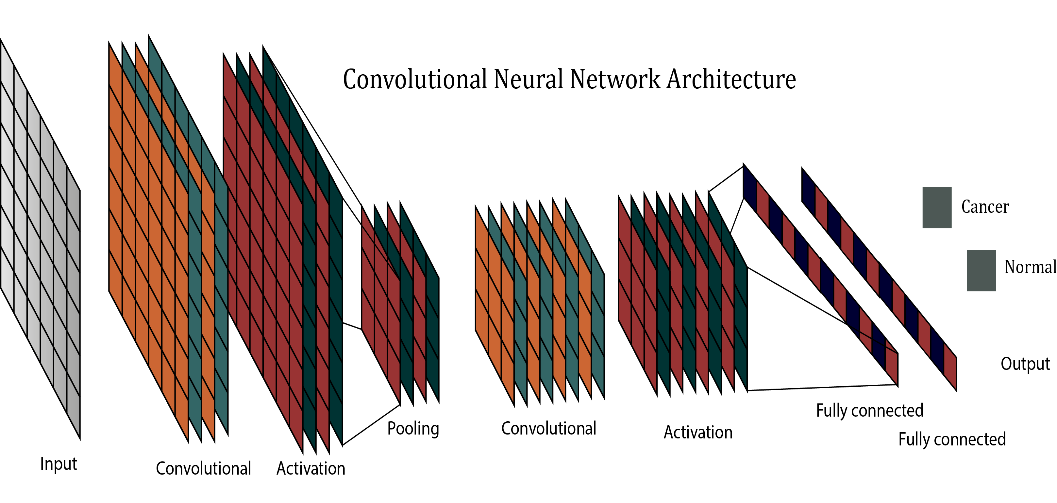
\includegraphics[width=14cm]{chaps/lr/cnn_arch}}
	\caption{معماری یک شبکه عصبی کانولوشنی}
	\label{fig:ch_lr:cnn_arch}
\end{figure}

همانطور که قبلاً بیان شد، \glspl{convnet} مدل‌های \gls{fullyconnectedffnn} هستند که از لایه‌های زیادی تشکیل شده اند. بسیاری از این مدل‌ها محدودیت‌های پارامتر و مکانی دارند که در ادامه توضیح داده خواهد شد. با این حال، آنها در تغییراتی که بر ورودی‌شان اعمال می‌کنند تفاوت دارند. در اینجا ما تمام لایه‌های یک شبکه کانولوشنی و توابع مورد استفاده در آموزش آن‌ها را شرح می‌دهیم. یک معماری می‌تواند یاد بگیرد که مسائل بسیار متفاوتی را حل کند تا زمانی که پارامترها برای هر یک از مسائل به خوبی بهینه شوند.

لایه ورودی فقط نمایشی از داده خام است که به مدل داده می‌شود که نیاز به شکل ورودی ثابت دارد. در رایج ترین حالت، یک تصویر به یک آرایه 3 \gls{dimension}ی تبدیل می‌شود با ابعاد [$w, h,3$] که $w$ و $h$ عرض و ارتفاع هستند. \gls{dimension} آخر به دلیل استفاده از تصاویر رنگی \lr{RGB\LTRfootnote{Red Green Blue}} اغلب $3$ است. وقتی از تصاویر \gls{xray} استفاده می‌کنیم چون دارای یک \gls{channel} \gls{intensity} هستند \gls{dimension} سوم برابر با $1$ است.

این لایه اصلی ترین لایه شبکه‌های عصبی کانولوشنی است و این شبکه‌ها نام‌ خود را از این لایه‌ها دریافت می‌کنند. وظیفه این لایه استخراج ویژگی‌ها است. این لایه عملیات کانولوشن را بر روی داده ورودی اعمال می‌کند و خروجی‌هایی به نام \gls{featuremap} از این لایه به دست می‌آید. در نتیجه تمامی نورون‌ها در یک \gls{featuremap}، وزن‌ها و \glspl{bias} مشابه و مشترکی دارند که باعث می‌شود، ویژگی‌های تصویر در موقعیت‌های مختلف قابل شناسایی باشند. از طرف دیگر این اشتراک وزن‌ها باعث کاهش تعداد پارامتر‌های مورد نیاز برای آموزش می‌شود. در شبکه‌های کانولوشن اتصالات به صورت نواحی کوچک و محلی صورت می‌گیرد. به بیان دیگر هر نورون در نخستین لایه مخفی به ناحیه کوچکی از نورون‌های ورودی متصل می‌شود. برای مثال اگر این ناحیه $5\times 5$ باشد این ناحیه کوچک $25$ پیکسلی \gls{localreceptivefield}  یا \gls{kernel} کانولوشن نامیده می‌شود. با توجه به شکل \ref{fig:ch_lr:cnn_conv5} یک تصویر ورودی $28\times 28$ داریم که یک \gls{kernel} $5\times 5$ بر روی پیکسل‌های ورودی از چپ به راست حرکت می‌کند هر پنجره به نورونی در لایه مخفی متصل می‌شود. بناباین همان طور که در شکل \ref{fig:ch_lr:cnn_conv5} مشخص است لایه مخفی شامل یک شبکه $24\times 24$ نورونی خواهد بود.

\begin{figure}[!ht]
	\centerline{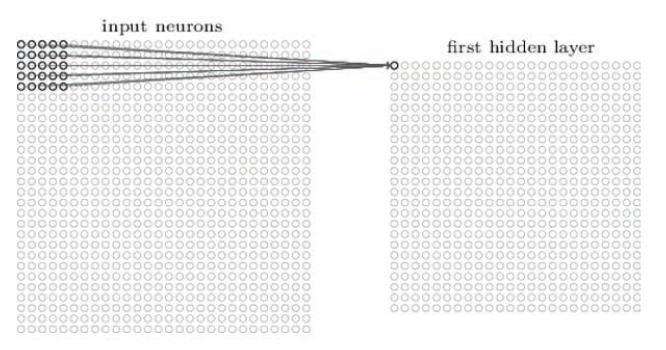
\includegraphics[width=11cm]{chaps/lr/cnn_conv5}}
	\caption{
		عملیات \gls{convolution} در یک \gls{convnet} با \gls{kernel} $5\times 5$
	}
	\label{fig:ch_lr:cnn_conv5}
\end{figure}

در شکل \ref{fig:ch_lr:cnn_conv5} هر نورون لایه مخفی دارای یک \gls{bias} و تعداد $5\times 5$ وزن می‌باشد که به  ناحیه ادراکی خود متصل شده است. تمامی نورون‌های لایه مخفی مذکور که دارای ابعاد $24\times 24$ هستند، دارای وزن‌ها و \glspl{bias}ی مشترکی می‌باشند. به عبارت دیگر خروجی نورون لایه کانولوشن $y_{w,h,m}$ در طول و عرض $w,h$ و عمق $m$ به صورت رابطه \ref{eq:ch_lr:neuron_ouput} است.
\begin{equation}
	y_{w,h,m} = f\left(\sum_{i=(w-1)S+1}^{(w-1)S+K} \sum_{j=(h-1)S+1}^{(h-1)S+K} \sum_{k=1}^{N} W_{k,m}(x_{i,j,k})+b_m\right)
	\label{eq:ch_lr:neuron_ouput}
%	\caption{خروجی نورون لایه کانولوشن}
\end{equation}

که در این رابطه $f$ \gls{activationfunction}، $b_m$ بایاس مشترک نورون‌ها، $W_{k,m}$ وز‌ن‌های $5\times 5$ مشترک نورون‌ها و $x_{i,j,k}$ ورودی در موقعیت $i,j,k$ می‌باشد. بنابراین تمامی نورون‌های واقع در لایه مخفی اول به طور دقیق ویژگی‌های مشابهی را در نواحی مختلف تصویر شناسایی می‌کنند. در نهایت خروجی لایه ورودی یا نورون‌های لایه مخفی به عنوان \gls{featuremap} شناخته می‌شوند. ابعاد مربوط به ماتریس خروجی لایه کانولوشن $W_2\times H_2 \times D_2$ که از ماتریس ورودی با ابعاد $W_1\times H_1 \times D_1$ است، به صورت رابطه \ref{eq:ch_lr:conv_ouput} به دست می‌آید.

\begin{equation}
	W_2 = \frac{W_1-F+2P}{S+1}, \qquad H_2=\frac{H_1-F+2P}{S+1}, \qquad D_2=K
	\label{eq:ch_lr:conv_ouput}
\end{equation}
در روابط \ref{eq:ch_lr:conv_ouput} که بیانگر نحوه محاسبه ابعاد ماتریس خروجی کانولوشن است،
$F, P, S$ و $k$
به ترتیب نشان دهنده اندازه \gls{kernel}، مدار \gls{zeropadding}، اندازه \gls{stride} و تعداد فیلترها می‌باشد. طبق این روابط به ازای هر فیلتر تعداد $F\times F\times D_1$ وزن داریم و با توجه به تعداد $k$ فیلتر موجود، در مجموع تعداد $k(F\times F\times D_1)$ وزن و $k$ بایاس ایجاد می‌شود. بنابراین تعداد پارامترهایی که شبکه در یک لایه کانولوشن خود می‌بایست آموزش ببیند زیاد است.

بکارگیری \gls{activationfunction} در لایه کانولوشن باعث ایجاد خصوصیات غیر خطی در خروجی می‌شود و باعث می‌شود عملکرد مدل متمایز کننده‌تر شود. این توابع با حفظ اندازه لایه، بدون نیاز به پارامترهای آموخته شده، یک عملكرد ساده عنصرگونه در مدل انجام می‌دهند. تابع \gls{relu} متداول ترین تابع مورد استفاده به خاطر آسان کردن مرحله آموزش است. مثال‌های دیگر شامل تابع \gls{sigmoid} و \gls{hyperbolictangent} است.
\begin{equation}
	\begin{aligned}
		\text{ReLU:}&\quad r_{m,n,c} = \max\{0,l_{x,y,z}\} \\
		\text{Sigmoid:}&\quad s_{m,n,c} = \frac{1}{1-\exp(-l_{x,y,z})}
	\end{aligned}
	\label{eq:ch_lr:relu-sigmoid}
\end{equation}
\begin{figure}[!ht]
	\centerline{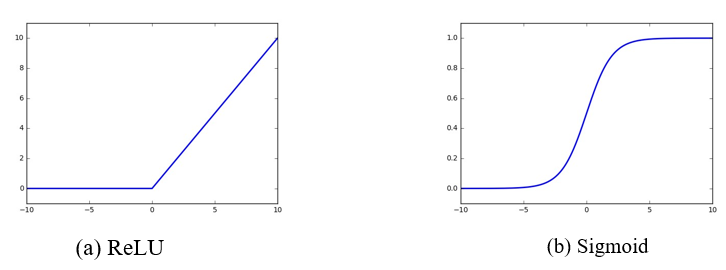
\includegraphics[width=14cm]{chaps/lr/activation_functions}}
	\caption{(\lr{a}) \gls{activationfunction} \lr{ReLU} و (\lr{b}) \gls{activationfunction} \gls{sigmoid}	
	}
	\label{fig:ch_lr:activation_functions}
\end{figure}
در یک شبکه عصبی کانولوشن معمولا پس از هر لایه کانولوشن یک لایه \lr{pooling} قرار می‌گیرد . این لایه‌ از آن جهت اهمیت دارد که باعث کاهش تعداد پارامترهایی می‌شود که باید آموزش ببینند. بنابراین با بکارگیری این لایه ضمن کاهش محاسبات مورد نیاز در بخش آموزش، باعث کنترل \gls{overfitting} احتمالی در شبکه می‌شود. این لایه بر روی هر عمق از ورودی اعمال می‌شود و اندازه آن را تغییر می‌دهد. دو تابع عملکردی معروف این لایه \lr{max-pooling} و \lr{mean-pooling} نام دارند که تابع اول دارای کاربرد بیشتری در \glspl{convnet} است. طریقه عملکرد \lr{max-pooling} به این صورت است که در هر پنجره بزرگترین \gls{pixel} را به خروجی می‌فرستد. این پنجره بر روی تصویر مانند تابع کانولوشن از چپ به راست و از بالا به پایین با انداه گام‌های مشخص حرکت می‌کند و نتیجه را به خروجی می‌فرستد. به دلیل اینکه این عملیات بر روی تمامی عمق‌ها اعمال می‌گردد، عمق خروجی همان عمق ورودی به لایه \lr{pooling} است. یک مثال از عمل \lr{max-pooling} در شکل \ref{fig:ch_lr:max_pooling} به نمایش گذاشته شده است.
\begin{equation}
	\text{with}\ l \in [s\times x, s\times x + m], j\in [s\times y, s\times y + m], \quad R_{x,y,x} = \max \{l_{i,j,z}\}
	\label{eq:ch_lr:max-pooling}
\end{equation}
\begin{figure}[!ht]
	\centerline{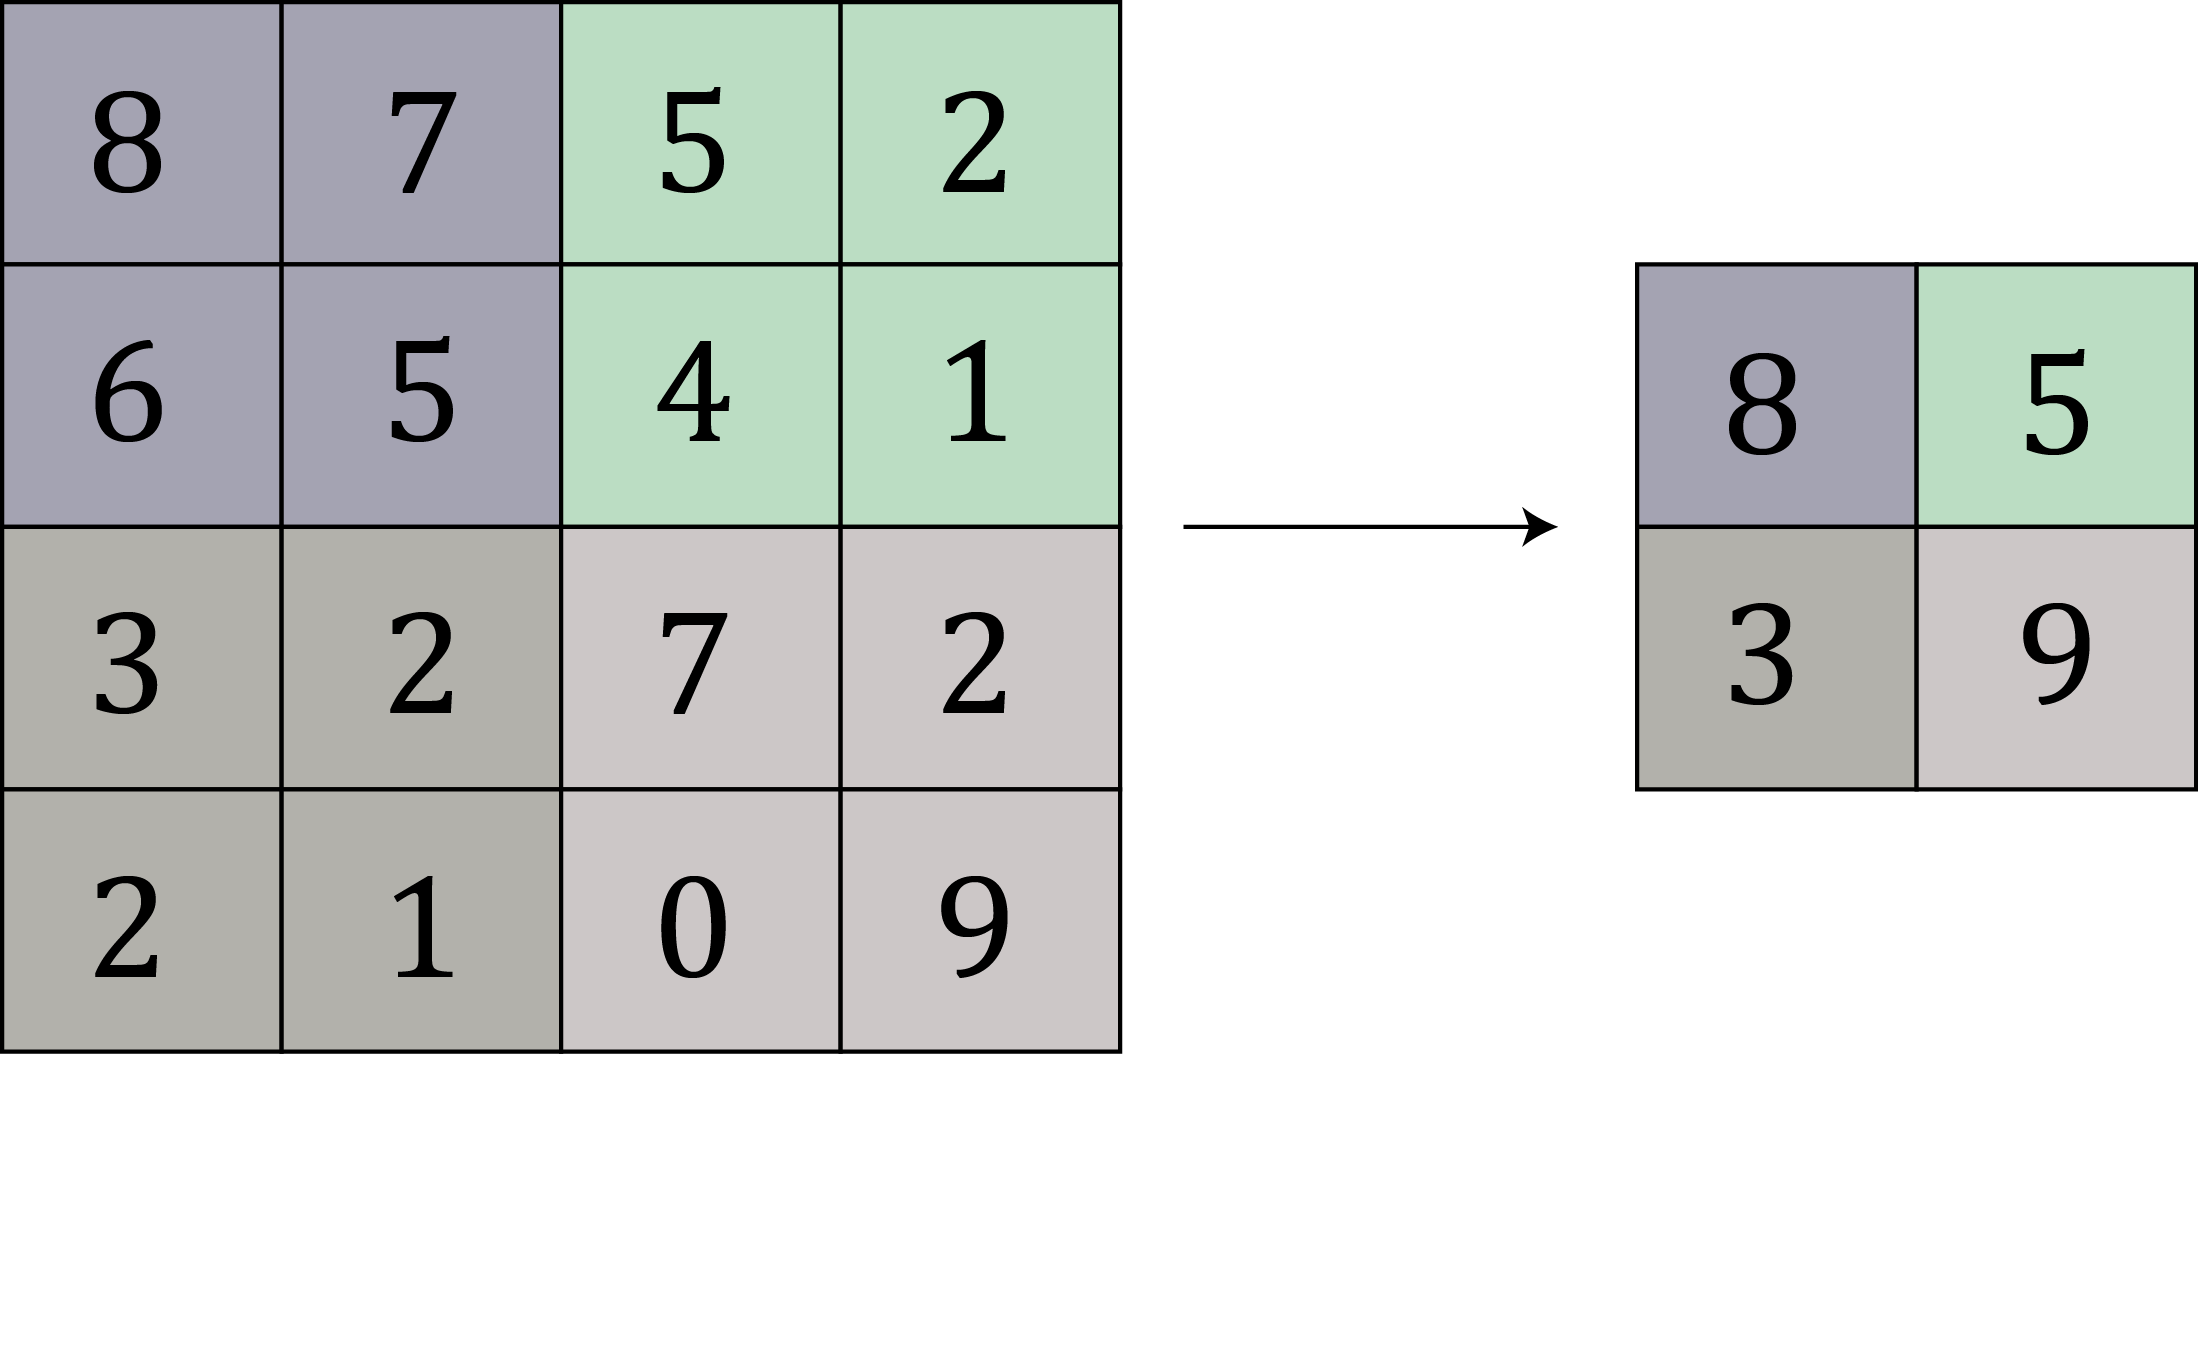
\includegraphics[width=8cm]{chaps/lr/max_pooling}}
	\caption{
		تابع \lr{max-pooling} بر روی آرایه دو بعدی کوچک $m=2$ و $s=2$
	}
	\label{fig:ch_lr:max_pooling}
\end{figure}
لایه کاملا متصل لایه آخر یک شبکه عصبی کانولوشنی محسوب می‌شود و اتصالات کاملی با خروجی لایه قبلی ایجاد می-کند. این لایه ورودی را دریافت و سپس خروجی را به صورت برداری با $N$ مولفه تولید می‌کند که $N$ تعداد کلاس‌هایی که شبکه باید طبقه بندی کند است. در واقع یک شبکه  \gls{convnet} جهت تولید یک بردار خروجی با $N$ مولفه عددی طراحی می‌شود که هر عدد در این بردار خروجی درصد احتمال تعلق به کلاس مورد نظر را نشان می‌دهد. برای یک مسئله با تعداد $k$  کلاس، $k$ نورون خروجی داریم که هر احتمال را با تابع \lr{SoftMax} محاسبه می‌کنند
\begin{equation}
	P(C)_j = \frac{e^{c_j}}{\sum^{K}_{k=1}e^{c_k}}
	\label{eq:ch_lr:softmax}
%	\caption{محاسبه احتمال هر کلاس با تابع \lr{SoftMax}}
\end{equation}
اگر دو کلاس داشته باشیم می‌توانیم از تابع \lr{SoftMax} با دو خروجی استفاده کنیم یا از یک نورون استفاده کنیم و تابع \gls{sigmoid} را محاسبه کنیم. برای دو کلاس احتمال توسط معادله \ref{binary_softmax} محاسبه می‌شود
\begin{equation}
	P(1) = \frac{1}{1+e^i} \qquad \qquad P(0) = 1-P(1)
	\label{eq:ch_lr:binary_softmax}
	%	\caption{احتمال کلاس1 و احتمال کلاس0}
\end{equation}
\gls{dropout} یک روش بسیار رایج برای جلوگیری از \gls{overfitting} شبکه عصبی مصنوعی از جمله مدل‌های \gls{deeplearning} است\cite{srivastava2014dropout}.
ایده این تکنیک این است که با جلوگیری از هماهنگی نورون‌ها ، ویژگی‌های قوی تری ایجاد شود. اجرای آن ساده است تنها نیاز به بهم چسباندن لایه‌های اضافی در شبکه معمولا پس از توابع فعال سازی است. این ماژول بطور تصادفی برخی از نقاط نقشه ویژگی ورودی را  صفر می‌کند. هریک از ماژول‌ها دارای یک احتمال مستقل $\sigma$ برای نگهداری نقاط هستند و در صورت بروز چنین اتفاقی ، توسط  $\frac{1}{\sigma}$ مقیاس بندی می‌شوند. نقاطی که نگهداری نمی‌شوند بر روی صفر تنظیم می‌شوند. این لایه فقط یک پارامتر $\sigma$ دارد، که برای آموزش در فاصله $[0,1]$ قرار دارد و برای آزمایش روی $1$ قرار می‌گیرد. به طور شهودی، می‌توان این فرآیند را به عنوان حذف برخی از نورون‌های شبکه عصبی ، به طور موقت ، همراه با اتصالات ورودی و خروجی آن تصور کرد. مکانیزم حذف، نورون‌هایی را که به اتصالات ورودی کمتری متکی هستند را در نظرمی‌گیرد. زیرا افت یک زیر مجموعه از ورودی‌ها در مقایسه با یک نورون که به بسیاری از ورودی‌ها متکی است، قابل توجه‌تر خواهد بود و به این ترتیب ویژگی‌های کلی‌تر مهم‌تر می‌شوند. شکل \ref{fig:ch_lr:dropout} یک مثال از لایه \gls{dropout} را نمایش می‌دهد.
\begin{figure}[!ht]
	\centerline{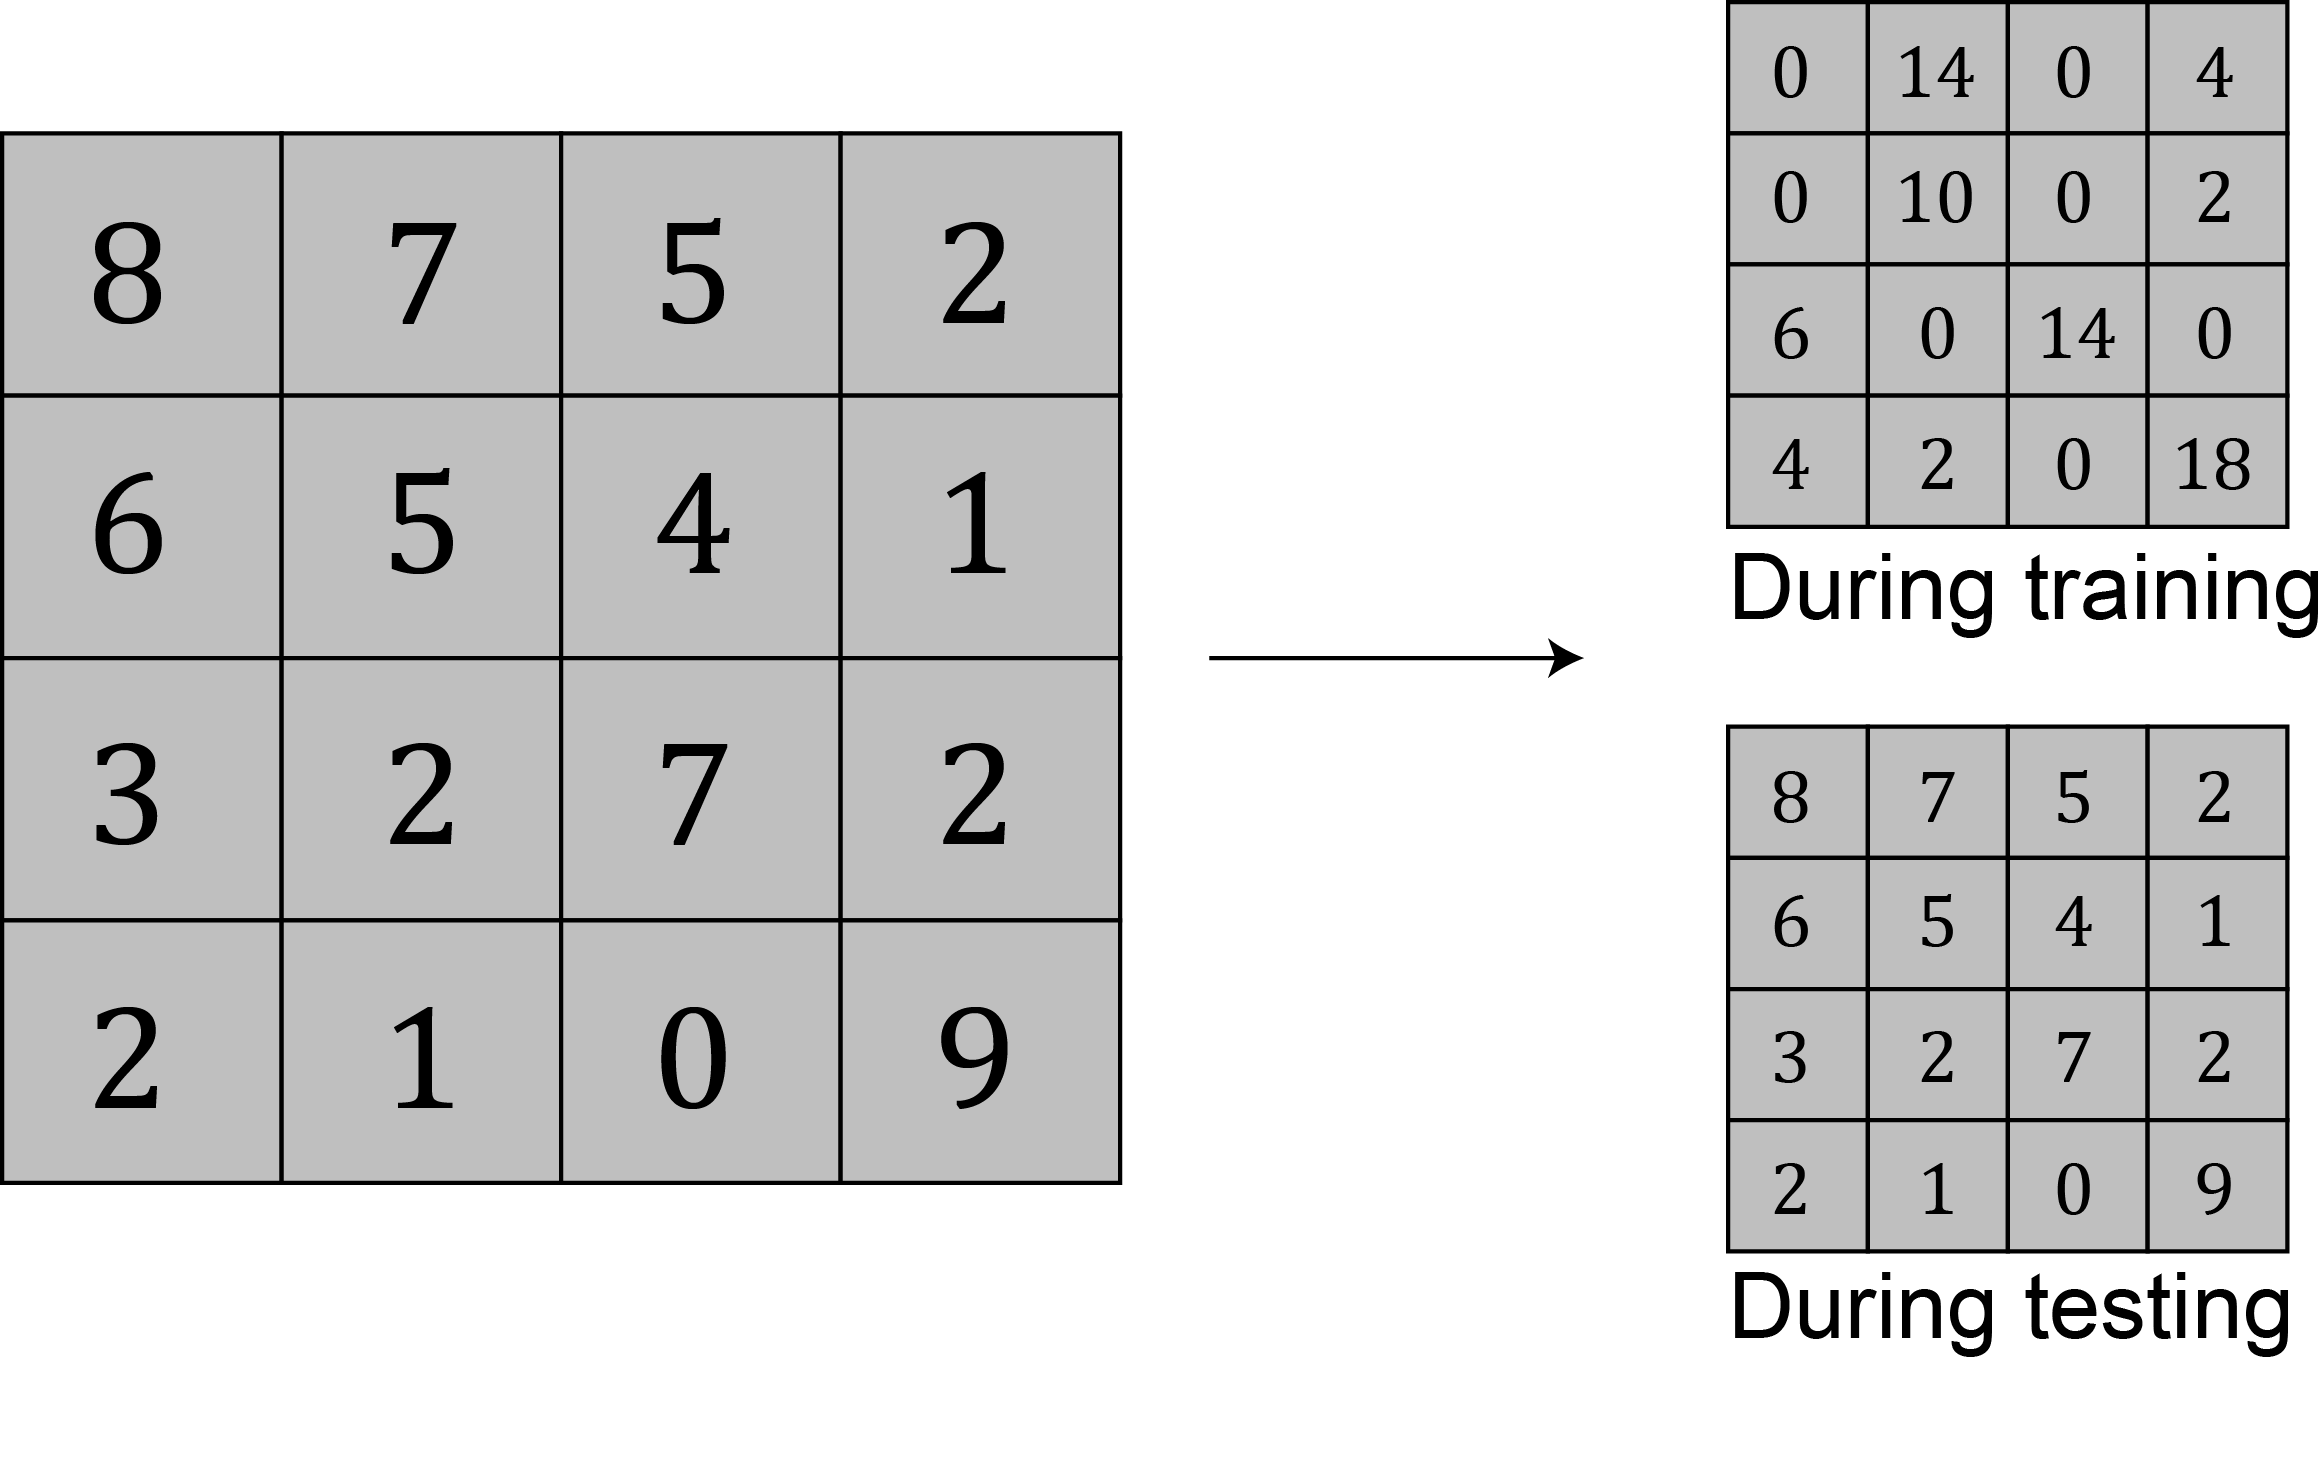
\includegraphics[width=10cm]{chaps/lr/dropout}}
	\caption{
	لایه \gls{dropout} با $\sigma=0.5$
	}
	\label{fig:ch_lr:dropout}
\end{figure}
\gls{batchnormalization} یک تکنیک جدید ولی خیلی کارامد است. در طی آموزش مدل‌های عمیق ، وزن‌ها در هر \gls{iteration}  به روز می‌شوند.
یک اثر جانبی این امر این است که در هر لایه توزیع‌های ورودی تغییر می‌کند، پدیده ای که به آن  \gls{internalcovariateshift}می‌گویند. این پدیده فرایند آموزش را کند می‌کند، به مقدار دهی دقیق‌تر وزن احتیاج دارد و مانع \gls{optimization} مدل‌های غیرخطی اشباع، مانند مماس‌های \gls{sigmoid} یا هایپربولیک می‌شود. برای حل این مشکل \gls{batchnormalization} را پیشنهاد می‌شود که مشابه با \gls{dropout}، به عنوان لایه ای در شبکه با رفتارهای متفاوت در حین آموزش و آزمون پیاده سازی می‌شود. برای رفع مشکل تغییر \gls{covariance} داخلی ، این لایه برای هر دسته آموزش  با کم کردن میانگین و تقسیم بر \gls{standarddeviation} همه نورون‌های عمق مشابه، ورودی خود را نرمال می‌کند. به میانگین و \gls{standarddeviation} آمار \lr{mini-batch}  گفته می‌شود. برای اطمینان از اینكه مدل می‌تواند دقیقاً همان تابع را با یا بدون \gls{batchnormalization} عادی نشان دهد ، دو وزن جدید قابل تمرین $\gamma$ و $\beta$ اضافه می‌شوند كه خروجی را اندازه گیری و جبران می‌كنند. بنابراین خروجی به صورت معادله \ref{eq:ch_lr:batch_normalization} است.
\begin{equation}
	\begin{aligned}
		\text{در طی آموزش}&: \quad I_c = \gamma \left(\frac{I_c-\text{\lr{mean}}(I_c)}{\text{\lr{std}}(I_c)}\right)+\beta  
		\\
		\text{در طی آزمایش}&: \quad I_c = \gamma \left(\frac{I_c-u_c}{v_c}\right)+\beta  
	\end{aligned}
	\label{eq:ch_lr:batch_normalization}
	%	\caption{احتمال کلاس1 و احتمال کلاس0}
\end{equation}
که $u_c$ و $v_c$ متوسط‌های در حال اجرا $\text{\lr{mean}}(I_c)$ و $\text{\lr{std}}(I_c)$ هستند. نشان داده شده است که \gls{batchnormalization} باعث آهنگ یادگیری بالاتر می‌شود و مدل در تکرارهای کمتری همگرا خواهد شد. این روش دارای اثر \gls{regularization} است. 
مدل با استفاده از \gls{costfunction} یاد می‌گیرد. این روشی است برای ارزیابی اینکه تا چه میزان خوب یک الگوریتم داده‌های مشاهده شده را می‌تواند مدل سازی کند. اگر پیش بینی‌ها بیش از حد از نتایج واقعی منحرف شوند ، \gls{costfunction} مقدار بالایی خواهد داشت. به تدریج، با کمک برخی توابع بهینه سازی، تابع هزینه می‌آموزد تا خطا در پیش بینی را کاهش دهد.

بهینه سازی مهمترین بخش در الگوریتم‌های یادگیری عمیق است. این کار با تعریف \gls{costfunction} شروع می‌شود و با به حداقل رساندن آن با استفاده از یک روش بهینه سازی به پایان می‌رسد. فرض کنید یک مجموعه داده $D$ با تعداد $I$ تصویر داریم. این تصاویر می‌توانند ضایعه باشند یا نباشند، بنابراین دارای برچسب $y\in \{0,1\}$ هستند.

باید مدلی بسازیم که با توجه به یک تصویر ورودی $I_i$، یک احتمال $p(I_i)$ تولید کند که تا حد ممکن به برچسب مربوط به آن تصویر ($y_i$) نزدیک باشد. برای این منظور الگوریتم‌های بهینه سازی متفاوتی وجو دارد مانند \lr{Adam}، \lr{SGD}\LTRfootnote{Stochastic gradient descent} و 
\lr{Adadelta}.\\
 به حداقل رساندن \gls{costfunction} با کاهش گرادیان تقریباً رایج ترین الگوریتم برای بهینه سازی شبکه‌‌های عصبی است. اگر \gls{costfunction} \gls{binarycrossentropy} باشد و بخواهیم محاسبه کنیم که $p(I_i)$ تا چه حد خوب می‌تواند برچسب $y_i$ را تقریب بزند از معادله \ref{eq:ch_lr:binary_ce} استفاده می‌شود.
 \begin{equation}
 	L = \frac{1}{|\mathcal{D}|}  \sum_i^{|\mathcal{D}|}\Big(y_i \log\big(P(I_i)\big) + (1-y_i) \log\big(1-P(I_i)\big)\Big)
 	\label{eq:ch_lr:binary_ce}
 	%	\caption{تابع خطا cross-entropy binary}
 \end{equation}
 احتمال برای یک ورودی به وزن‌های آن ($\theta$) بستگی دارد و با
 $p(I, \theta)$ 
 نمایش داده می‌شود. با توجه به $\theta$ می‌توان $L(\theta)$ را با اجرای مدل بر روی مجموعه داده به دست آورد.
 
 \gls{backpropagation}
 اساس آموزش شبکه عصبی است. این عمل تنظیم-دقیق  وزن‌های یک شبکه عصبی بر اساس میزان \gls{loss} در هر \gls{epoch} قبلی است که این امر با محاسبه مشتق‌های تابع خطا بر اساس وزن‌ها 
 $\nabla_\theta L(\theta)$
 در زمان آموزش امکان پذیراست. تنظیم مناسب وزن‌ها  باعث کاهش میزان خطا می‌شود. در فرایند \gls{backpropagation}  ابتدا ورودی در سراسر شبکه انتشار داده می‌شود سپس $L(\theta)$ محاسبه شده و در نهایت این \gls{loss} از طریق تمام وزن‌ها در شبکه رو به عقب منتشر می‌شود. مشتق \gls{costfunction} از خروجی توسط معادله \ref{eq:ch_lr:dif_cf} محاسبه می‌شود.
 \begin{equation}
 	\frac{\partial L}{\partial P} = \frac{\partial \Big(-\big(y_i \log(p) + (1-y)\log(1-P)\big)\Big)}{\partial P} = \frac{P-y}{P(1-P)}
 	\label{eq:ch_lr:dif_cf}
 	%	\caption{محاسبه مشتق از تابع هزینه}
 \end{equation}
 همچنین محاسبه مشتق \gls{costfunction} $L$ از ورودی $i$ به صورت معادله \ref{eq:ch_lr:dif_cf_i} محاسبه می‌شود.
  \begin{equation}
 	\frac{\partial L}{\partial i} = \frac{\partial L}{\partial P} \frac{\partial P}{\partial i} = P-y
 	\label{eq:ch_lr:dif_cf_i}
 \end{equation}
 همچنین محاسبه مشتق \gls{costfunction} بر اساس وزن‌های لایه آخر $w$ به صورت، 
   \begin{equation}
 	\frac{\partial L}{\partial w} = \frac{\partial L}{\partial P} \frac{\partial P}{\partial i}  \frac{\partial i}{\partial w}= (P-y)a
 	\label{eq:ch_lr:dif_cf_w}
 \end{equation}
 می‌باشد که $a$ در آن برابر با ترکیب خطی از ورودی‌های لایه آخر است. این کار را می‌توان به راحتی به لایه‌های قبلی تعمیم داد، بنابراین می‌توان $\nabla _\theta L(\theta)$ را محاسبه کرد.
 \section{شبکه‌های عصبی بازگشتی}
 قبل از آشنا شدن با \glspl{rnn} بهتر است مروری بر مفهوم شبکه عصبی داشته باشیم. شبکه‌های عصبی مجموعه‌ای از الگوریتم‌ها هستند که شباهت نزدیکی به مغز انسان داشته و به منظور تشخیص الگوها طراحی شده‌اند. شبکه‌ی عصبی داده‌های حسی را از طریق ادراک ماشینی ، برچسب زدن یا خوشه بندی ورودی‌های خام تفسیر می‌کند. شبکه می‌تواند الگوهای عددی را شناسایی ‌کند؛ این الگوها بردارهایی هستند که همه‌ی داده‌های دنیای واقعی (تصویر، صدا، متن یا سری‌های زمانی) برای تفسیر باید به شکل آن‌ها درآیند. شبکه‌های عصبی مصنوعی از تعداد زیادی مؤلفه‌ی پردازشی (نورون) تشکیل شده‌اند که اتصالات زیادی بینشان وجود دارد و برای حل یک مسئله با یکدیگر همکاری دارند.
 شبکه‌ی عصبی مصنوعی معمولاً تعداد زیادی پردازشگر دارد که به صورت موازی کار می‌کنند و در ردیف‌هایی کنار هم قرار می‌گیرند. ردیف اول، همچون عصب‌های بینایی انسان در پردازش بصری، اطلاعات ورودی‌های خام را دریافت می‌کند. سپس هر کدام از ردیف‌های بعدی، به جای ورودی خام، خروجی ردیف قبلی را دریافت می‌کنند؛ در پردازش بصری نیز نورون‌هایی که از عصب بینایی فاصله دارند، سیگنال را از نورون‌های نزدیک‌تر می‌گیرند. ردیف آخر خروجی کل سیستم را تولید می‌کند.

\subsection{شبکه عصبی بازگشتی چیست؟}
 شبکه‌ی عصبی بازگشتی شکلی از شبکه‌ی عصبی پیشخور است که یک حافظه‌ی داخلی دارد. شبکه عصبی بازگشتی ذاتاً بازگشتی است، زیرا یک تابع یکسان را برای همه‌ی داده‌های ورودی اجرا می‌کند، اما خروجی داده‌ی (ورودی) فعلی به محاسبات ورودی قبلی بستگی دارد. خروجی بعد از تولید، کپی شده و مجدداً به شبکه‌ی بازگشتی فرستاده می‌شود. این شبکه برای تصمیم‌گیری، هم ورودی فعلی و هم خروجی که از ورودی قبلی آموخته شده را در نظر می‌گیرد.
 شبکه عصبی بازگشتی برخلاف شبکه‌های عصبی پیشخور می‌توانند از حالت (حافظه‌ی) درونی خود برای پردازش دنباله‌هایی از ورودی‌ها استفاده کنند. این خاصیت باعث می‌شود در مسائلی همچون تشخیص دست‌خط زنجیره‌ای یا تشخیص گفتار کاربرد داشته باشند. در سایر شبکه‌های عصبی، ورودی‌ها از یکدیگر مستقل هستند، اما در شبکه عصبی بازگشتی ورودی‌ها به هم مرتبط می‌باشند. به شکل \ref{fig:ch_lr:rnn} توجه کنید،
 \begin{figure}[!ht]
 	\centerline{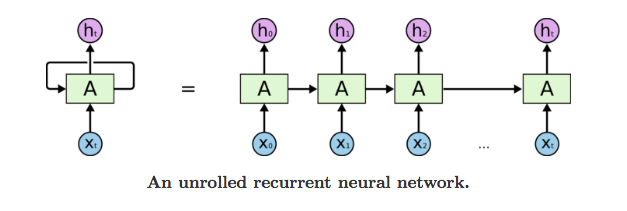
\includegraphics[width=14cm]{chaps/lr/rnn}}
 	\caption{
 		یک نمونه بازشده \gls{rnn}
 	}
 	\label{fig:ch_lr:rnn}
 \end{figure}
 این شبکه ابتدا $X_0$ را از دنباله‌ی ورودی‌ها گرفته و خروجی $h_0$ را تولید می‌کند که همراه با $X_1$ ورودی گام بعدی محسوب خواهند شد. یعنی $h_0$ و $X_1$ ورودی گام بعدی هستند. به همین صورت $h_1$ بعدی همراه با $X_1$ ورودی گام بعدی خواهند بود. شبکه عصبی بازگشتی بدین طریق می‌تواند هنگام آموزش زمینه را به خاطر داشته باشد.
 فرمول \gls{state} کنونی به صورت رابطه \ref{eq:ch_lr:rnn_cs} خواهد بود که در آن،
 \begin{equation}
 	h_t = f(h_{t-1}, x_t)
 	\label{eq:ch_lr:rnn_cs}
 \end{equation}
 خواهد بود که در آن $h_t$ برابر است با،
 \begin{equation}
 	h_t = \tanh(W_{hh}h_{t-1} + W_{hx}x_t)
 	\label{eq:ch_lr:rnn_ht}
 \end{equation}
 در این فرمول $W$ وزن، $h$ تک‌بردار نهان، $W_hh$ وزن حالت نهان قبلی، $W_{hx}$ وزن حالت ورودی کنونی و $\tanh$ \gls{activationfunction} است که با استفاده از تابعی غیرخطی، خروجی را فشرده می‌کند تا در بازه‌ی $[1, -1]$ جای گیرند. در نهایت \gls{state} خروجی $Y_t$ از طریق رابطه \ref{eq:ch_lr:rnn_hy} بدست می‌آید،
 \begin{equation}
 	y_t = W_{hy}h_t
 	\label{eq:ch_lr:rnn_hy}
 \end{equation}
 که در آن $W_{hy}$ برابر وزن در \gls{state} تولید شده را نشان می‌دهد.
 
 \subsection{مزایای \gls{rnn}}
 شبکه عصبی بازگشتی می‌تواند دنباله‌ای از داده‌ها را به شکلی مدل‌سازی کند که هر نمونه وابسته به نمونه‌های قبلی به نظر برسد. شبکه عصبی بازگشتی را می‌توان با لایه‌های پیچشی نیز به کار برد تا گستره‌ی همسایگی پیکسلی را افزایش داد.
 
 \subsection{معایب \gls{rnn}}
 \begin{itemize}
 	\item گرادیان کاهشی و مشکلات ناشی از آن
 	\item آموزش بسیار دشوار
 	\item ناتوانی در پردازش دنباله‌های طولانی از ورودی در صورت استفاده از \gls{activationfunction}  $\tanh$ یا \lr{ReLU}
 \end{itemize}

\subsection{کاربردهای \gls{rnn}}
\begin{itemize}
	\item شرح نویسی عکس\LTRfootnote{Image Captioning}: شبکه عصبی بازگشتی با تحلیل حالت کنونی عکس، برای شرح نویسی عکس به کار می‌رود
	\item پیش بینی سری‌های زمانی\LTRfootnote{Time Series Prediction}: هر مسئله سری زمانی مانند پیش بینی قیمت یک سهام در یک ماه خاص، با \gls{rnn} قابل انجام است
	\item
	پردازش زبان طبیعی\LTRfootnote{Natural Language Processing}: کاوش متن و تحلیل احساسات می‌تواند با استفاده از \gls{rnn} انجام شود
	\item
	ترجمه ماشینی\LTRfootnote{Machine Translation}: شبکه \gls{rnn} می‌تواند ورودی خود را از یک زبان دریافت و آن را به عنوان خروجی به زبان دیگری ترجمه کند
\end{itemize}
 
\subsection{انواع \gls{rnn}}
\noindent
 به طور کلی 4 نوع شبکه عصبی بازگشتی داریم:\\
 یک به یک (\lr{one to one}) : این نوع شبکه عصبی به عنوان شبکه عصبی وانیلی نیز شناخته می‌شود و برای مسائل یادگیری ماشین که یک ورودی و یک خروجی دارند به کار می‌رود.

 \begin{figure}[!ht]
 	\centering
 	\subfloat[یک به یک]{
 		\centering
 		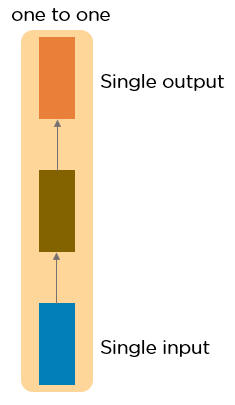
\includegraphics[width=0.17\textwidth]{chaps/lr/rnn_oto}
 		\label{fig:ch_lr:rnn_oto}
 	}
 	\hfill
 	\subfloat[یک به چند]{
 		\centering
 		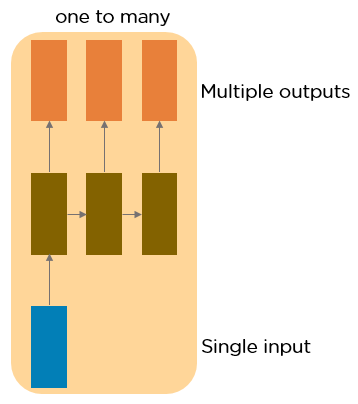
\includegraphics[width=0.26\textwidth]{chaps/lr/rnn_otm}
 		\label{fig:ch_lr:rnn_otm}
 	}
 	\hfil
 	\subfloat[چند به یک]{
 		\centering
 		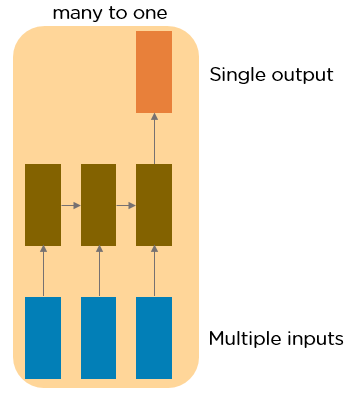
\includegraphics[width=0.26\textwidth]{chaps/lr/rnn_mto}
 		\label{fig:ch_lr:rnn_mto}
 	} 	\hfill
 	\subfloat[چند به چند]{
 		\centering
 		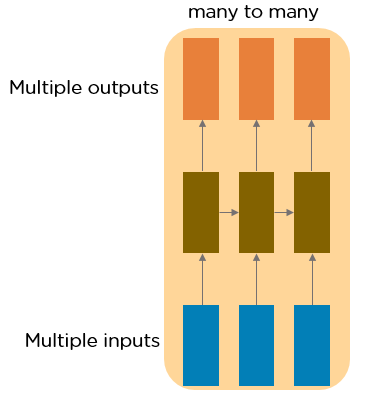
\includegraphics[width=0.26\textwidth]{chaps/lr/rnn_mtm}
 		\label{fig:ch_lr:rnn_mtm}
 	}
 	\caption{ساختار \gls{rnn}}
 	\label{fig:ch_lr:rnn_xtx}
 \end{figure}
 
% 
% \begin{figure}[!ht]
% 	\centerline{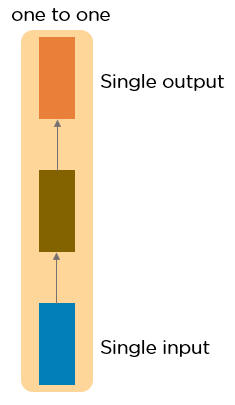
\includegraphics[width=4cm]{chaps/lr/rnn_oto}}
% 	\caption{ساختار \gls{rnn} یک به یک}
% 	\label{fig:ch_lr:rnn_oto}
% \end{figure}
%\\
 یک به چند (\lr{one to many}): این شبکه عصبی بازگشتی دارای یک ورودی و چند خروجی است. یک نمونه آن، شرح نویسی عکس است.
% \begin{figure}[!ht]
% 	\centerline{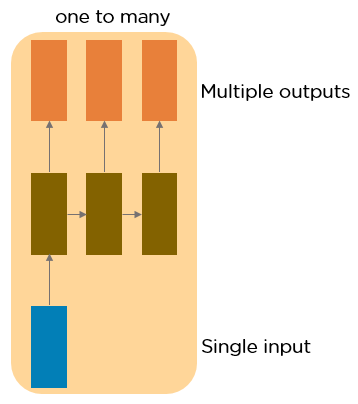
\includegraphics[width=7cm]{chaps/lr/rnn_otm}}
% 	\caption{ساختار \gls{rnn} یک به چند}
% 	\label{fig:ch_lr:rnn_otm}
% \end{figure}
\\

 چند به یک (\lr{many to one}): این نوع از \gls{rnn}، دنباله ایی از ورودی ها را می‌گیرد و یک خروجی تولید می‌کند. تحلیل احساسات مثال خوبی از این نوع شبکه است که یک جمله را به عنوان ورودی می‌گیرد و آن را با احساس مثبت یا منفی طبقه بندی می‌کند.

%
% \begin{figure}[!ht]
% 	\centerline{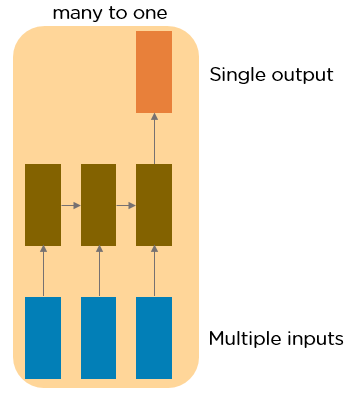
\includegraphics[width=7cm]{chaps/lr/rnn_mto}}
% 	\caption{ساختار \gls{rnn} چند به یک}
% 	\label{fig:ch_lr:rnn_mto}
% \end{figure}
 
 چند به چند (\lr{many to many}): دنباله ایی از ورودی ها را می‌گیرد و دنباله ایی از خروجی ها را تولید می‌کند. ترجمه ماشینی نمونه ایی از این نوع شبکه است.
%\begin{figure}[!ht]
%	\centerline{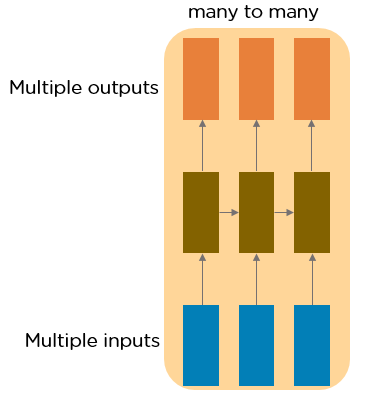
\includegraphics[width=7cm]{chaps/lr/rnn_mtm}}
%	\caption{ساختار \gls{rnn} چند به چند}
%	\label{fig:ch_lr:rnn_mtm}
%\end{figure} 


 \subsection{حافظه‌ی کوتاه‌مدت بلند (\lr{LSTM})}
 شبکه‌های \gls{lstm} یا \lr{LSTM} نسخه‌ی تغییریافته‌ای از شبکه‌های عصبی بازگشتی هستند که یادآوری داده‌های گذشته در آن‌ها تسهیل شده است. مشکل گرادیان کاهشی که در شبکه عصبی بازگشتی وجود داشت نیز در این شبکه‌ها حل شده است. شبکه‌های \lr{LSTM} برای مسائل رده‌بندی، پردازش و پیش‌بینی سری‌های زمانی با استفاده از برچسب‌های زمانی مدت‌های نامعلوم مناسب هستند. این شبکه‌ها مدل را با استفاده از انتشار رو به عقب آموزش می‌دهند. 
 \begin{figure}[!ht]
 	\centerline{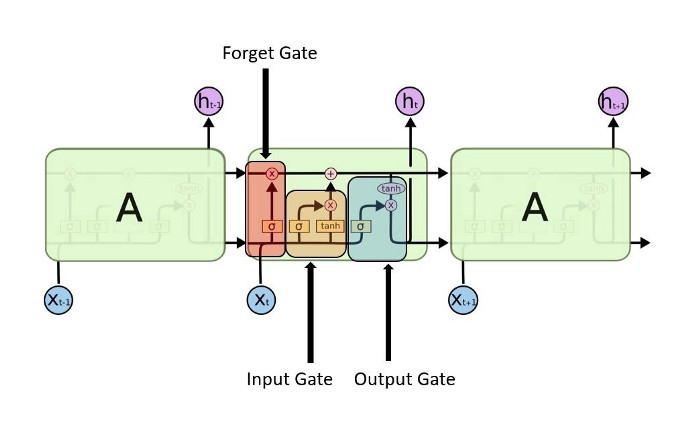
\includegraphics[width=15cm]{chaps/lr/lstm}}
 	\caption{ساختار \lr{LSTM}}
 	\label{fig:ch_lr:lstm}
 \end{figure}
\\
همان‌طور که در شکل \ref{fig:ch_lr:lstm} نمایش داده شده است، در یک شبکه‌ی \lr{LSTM} سه دریچه وجود دارد:
 
\subsubsection*{دریچه‌های \lr{LSTM}}
\textbf{1) دریچه‌ی ورودی}:
با استفاده از این دریچه می‌توان دریافت کدام مقدار از ورودی را باید برای تغییر حافظه به کار برد. تابع \gls{sigmoid} تصمیم می‌گیرد مقادیر بین $0$ و $1$ اجازه‌ی ورود دارند و تابع $\tanh$ با ضریب‌دهی (بین $-1$ تا $+1$) به مقادیر، در مورد اهمیت آن‌ها تصمیم می‌گیرد.
 \begin{equation}
  	\begin{aligned}
  		i_t &= \sigma (W_i \cdot [h_{t-1}, x_t]+b_i)
  		\\
  		\tilde{C}_t &= \tanh(W_C \cdot [h_{t-1}, x_t] + b_C)
  	\end{aligned}
 	\label{eq:ch_lr:lstm_in}
 \end{equation}
 
\textbf{2) دریچه‌ی فراموشی}:
 از طریق این دریچه می‌توان جزئیاتی را که باید از بلوک حذف شوند، تشخیص داد. تصمیم‌گیری در این مورد برعهده‌ی تابع \gls{sigmoid} است. این تابع با توجه به حالت قبلی $h_{t-1}$ و ورودی محتوا $X_t$، عددی بین $0$ تا $1$ به هرکدام از اعداد موجود در حالت سلولی $C_{t-1}$ اختصاص می‌دهد؛ $0$ نشان‌دهنده‌ی حذف آن عدد و $1$ به معنی نگه داشتن آن است.
 \begin{equation}
	f_t = \sigma(W_f\cdot [h_{t-1}, x_t] + b_f)
 	\label{eq:ch_lr:lstm_loss}
 \end{equation}
 
\textbf{3) دریچه‌ی خروجی}:
 ورودی و حافظه‌ی بلوک برای تصمیم‌گیری در مورد خروجی مورد استفاده قرار می‌گیرند. تابع سیگموئید تصمیم می‌گیرد مقادیر بین $0$ و $1$ اجازه‌ی ورود دارند و تابع $\tanh$ با ضریب‌دهی (بین $-1$ تا $+1$) به مقادیر و ضرب آن‌ها در خروجی تابع \gls{sigmoid} در مورد اهمیت آن‌ها تصمیم‌گیری می‌کند.
 \begin{equation}
 	\begin{aligned}
 		o_t &= \sigma (W_o \cdot [h_{t-1}, x_t]+b_o)
 		\\
 		h_t &= o_t \ast \tanh(C_t)
 	\end{aligned}
 	\label{eq:ch_lr:lstm_out}
 \end{equation}

 در حقیقت هدف از طراحی شبکه‌های \lr{LSTM}، حل کردن مشکل وابستگی بلندمدت بود. به این نکته مهم توجه کنید که به یاد سپاری اطلاعات برای بازه‌های زمانی بلند مدت، رفتار پیش‌فرض و عادی شبکه‌های \lr{LSTM} است و ساختار آ‌ن‌ها به صورتی است که اطلاعات خیلی دور را به خوبی یاد می‌گیرند که این ویژگی در ساختار آن‌ها نهفته است.
 
 همه شبکه‌های عصبی بازگشتی به شکل دنباله‌ای (زنجیره‌ای) تکرار شونده از ماژول‌های (واحد‌های) شبکه‌های عصبی هستند. در شبکه‌های عصبی بازگشتی استاندارد، این ماژول‌های تکرار شونده ساختار ساده‌ای دارند، برای مثال تنها شامل یک لایه تانژانتِ هایپربولیک ($\tanh$) هستند.
 
 \begin{figure}[!ht]
 	\centerline{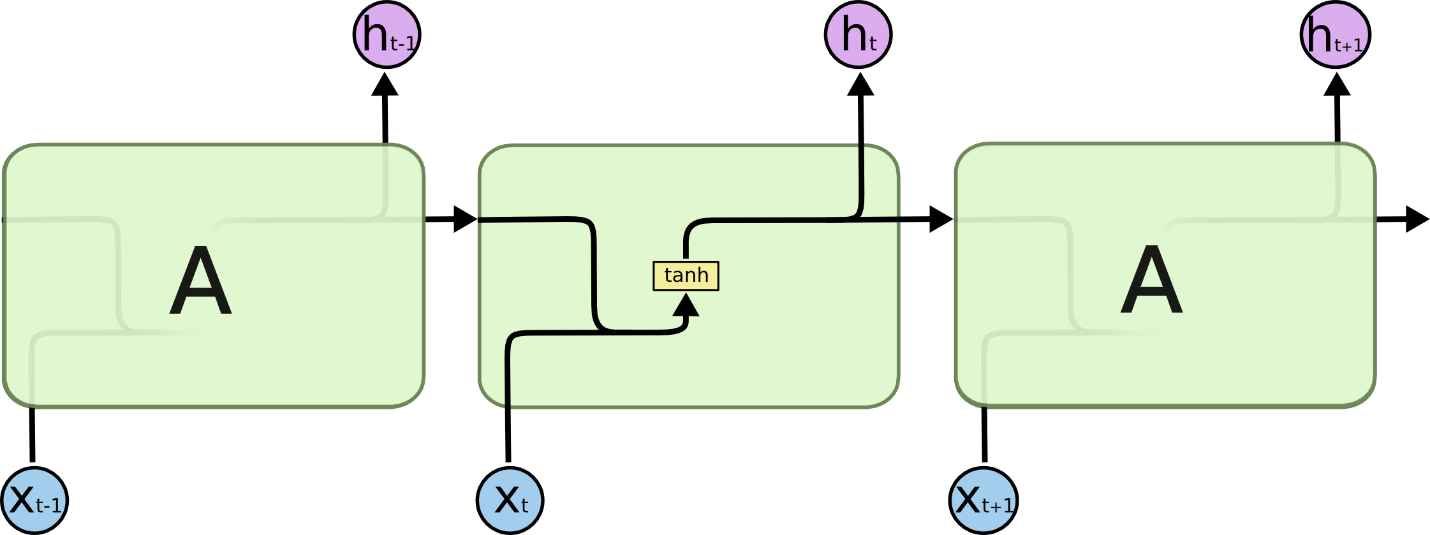
\includegraphics[width=14cm]{chaps/lr/rnn_chain}}
 	\caption{
ماژول‌های تکرار شونده در شبکه‌های عصبی بازگشتی استاندارد فقط دارای یک لایه هستند.
 	}
 	\label{fig:ch_lr:rnn_chain}
 \end{figure}
 
 شبکه‌های \lr{LSTM} نیز چنین ساختار دنباله یا زنجیره‌مانندی دارند ولی ماژولِ تکرار شونده ساختار متفاوتی دارد. به جای داشتن تنها یک لایه شبکه عصبی، 4 لایه دارند که طبق ساختار ویژه‌ای با یکدیگر در تعامل و ارتباط هستند.
 \begin{figure}[!ht]
	\centerline{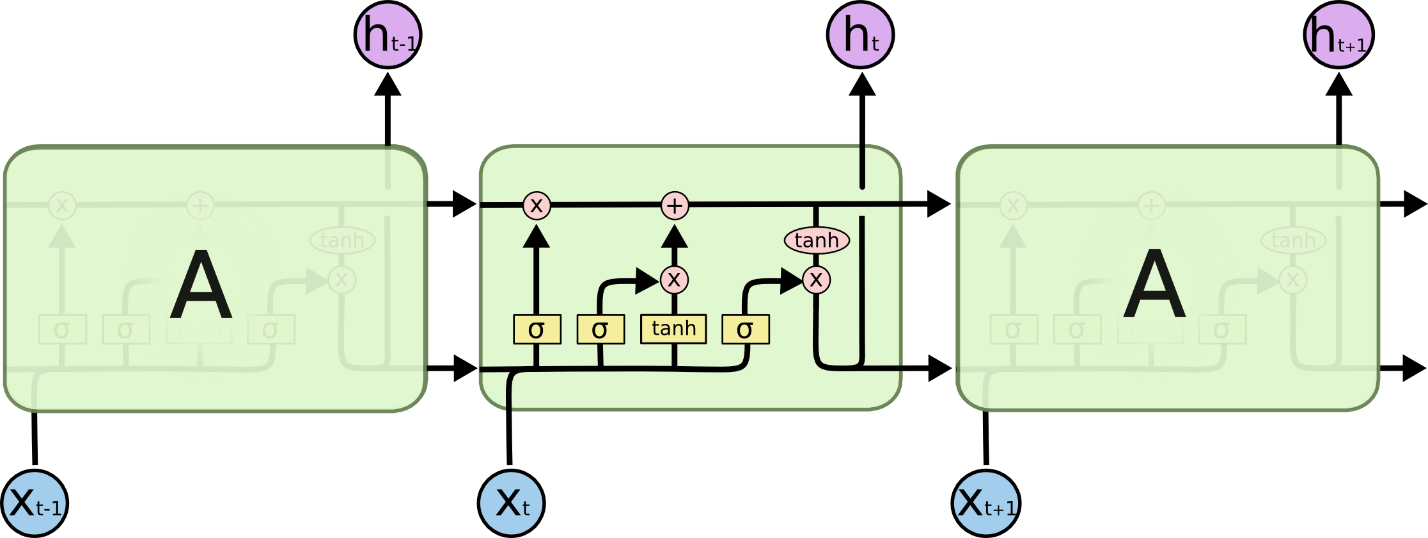
\includegraphics[width=14cm]{chaps/lr/rnn_inside}}
	\caption{
		ماژول‌های تکرار شونده در \lr{LSTM}ها دارای 4 لایه هستند که با هم در تعامل می‌باشند.
	}
	\label{fig:ch_lr:rnn_inside}
\end{figure} 
در ادامه قدم به قدم ساختار شبکه‌های \gls{lstm} را توضیح خواهیم داد. اما در ابتدا معنی هر کدام از شکل‌ و علامت‌هایی را که از آن‌ها استفاده خواهیم کرد توضیح می‌دهیم.
  \begin{figure}[!ht]
 	\centerline{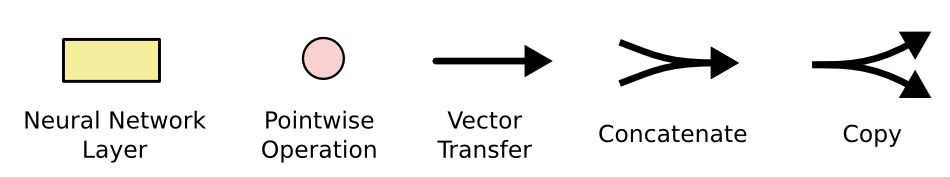
\includegraphics[width=14cm]{chaps/lr/lstm_legend}}
 	\caption{
 		اشکال از راست به چپ به تریب برابر هستند با: کپی کردن، وصل کردن، بردار انتقال، عملیات نقطه به نقطه، یک لایه‌ی شبکه عصبی.
 	}
 	\label{fig:ch_lr:lstm_legend}
 \end{figure} 
 در شکل \ref{fig:ch_lr:lstm_legend}، هر خط یک بردار را به صورت کامل از خروجی یک گره به ورودی گره دیگر انتقال می‌دهد. دایره‌های صورتی نمایش دهنده عملیات‌های نقطه‌ به نقطه مانند «جمع کردن دو بردار» هستند. مستطیل‌های زرد، لایه‌‌های شبکه‌های عصبی هستند که شبکه پارامتر‌های آن‌ها را یاد می‌گیرد. خط‌هایی که با هم ادغام می‌شوند نشان‌دهنده \gls{concatenation} و خط‌هایی که چند شاخه می‌شوند نشان دهنده‌ای این موضوع است که محتوای آن‌ها کپی و به بخش‌های مختلف ارسال می‌شود.
\\
\\
 عنصر اصلی \lr{LSTM}ها سلول حالت\LTRfootnote{Cell state} است که در حقیقت یک خط افقی است که در بالای شکل \ref{fig:ch_lr:lstm_cellState1} قرار دارد.
 سلول حالت را می‌توان به صورت یک تسمه نقاله تصور کرد که از اول تا آخر دنباله یا همان زنجیره با تعاملات خطیِ جزئی در حرکت است (یعنی ساختار آن بسیار ساده است و تغییرات کمی در آن اتفاق می‌افتد).
   \begin{figure}[!ht]
 	\centerline{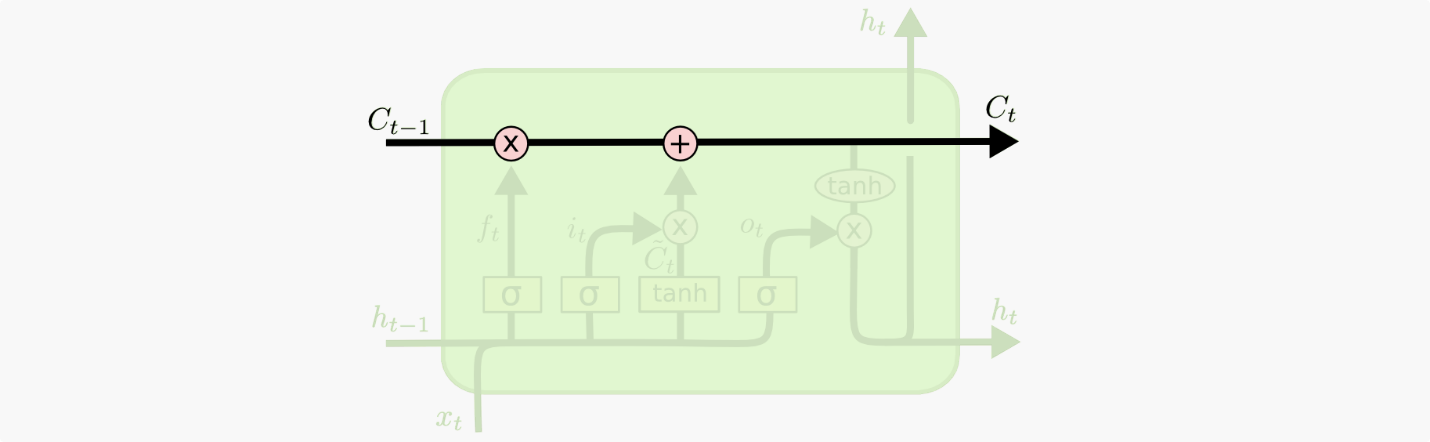
\includegraphics[width=15cm]{chaps/lr/lstm_cellState1}}
 	\caption{
 		سلول حالت در ماژول \lr{LSTM}
 	}
 	\label{fig:ch_lr:lstm_cellState1}
 \end{figure} 
\\
 \lr{LSTM} 
 این توانائی را دارد که اطلاعات جدیدی را به سلول حالت اضافه یا اطلاعات آن را حذف کنید. این کار توسط ساختارهای دقیقی به نام \glspl{gate} انجام می‌شود. \glspl{gate}‌ راهی هستند برای ورود اختیاری اطلاعات. آن‌ها از یک لایه شبکه عصبیِ \gls{sigmoid} به همراه یک عملگر ضرب نقطه به نقطه تشکلیل شده‌اند.
 \begin{figure}[!ht]
 	\centerline{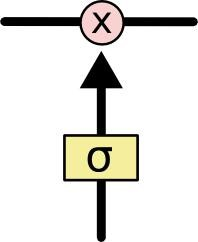
\includegraphics[width=3cm]{chaps/lr/lstm_2}}
 	\caption{
 		نمایی از نحوه تاثیر و ورود اطلاعات به سلول حالت
 	}
 	\label{fig:ch_lr:lstm_2}
 \end{figure} 
\\
 خروجی لایه \gls{sigmoid} عددی بین صفر و یک است، که نشان می‌دهد چه مقدار از وروی باید به خروجی ارسال شود. مقدار صفر یعنی هیچ اطلاعاتی نباید به خروجی ارسال شود در حالی که مقدار یک یعنی تمام ورودی به خروجی ارسال شود!
 \\
 \\
 \lr{LSTM}
  دارای 3 \gls{gate} مشابه برای کنترل مقدار سلول حالت است که در ادامه به بررسی قدم به قدمِ آن‌ها از لحظه ورود تا خروج اطلاعات خواهیم پرداخت.
  \\
 قدم اول در \lr{LSTM} تصمیم در مورد اطلاعاتی است که می‌خواهیم آن‌ها را از سلول حالت پاک کنیم. این تصمیم توسط یک لایه \gls{sigmoid} به نام «دروازه فراموشی\LTRfootnote{Forget gate}» انجام می‌شود. این \gls{gate} با توجه به مقادیر $h_{t-1}$ و $x_t$، برای هر عدد، مقدار صفر یا یک را در سلول حالتِ $C_{t-1}$ به خروجی می‌برد. مقدار یک یعنی به صورت کامل مقدار حال حاضرِ سلول حالت $C_{t-1}$ را به $C_t$ انتقال داده شود و مقدار صفر یعنی به صورت کامل اطلاعات سلول حالت کنونی $C_{t-1}$ را پاک شود و هیچ مقداری از آن  به $C_t$ برده نشود. بیاید به مثال قبلی‌مان که یک مدل زبانی‌ای بود که در آن تلاش داشتیم کلمه بعدی را بر اساس همه کلمه‌های قبلی حدس بزنیم، برگردیم. در چنین مسأله‌ای، سلول حالت ممکن است دربردارنده جنسیت فاعل کنونی باشد، که با توجه به آن می‌توانیم تشخیص دهیم از چه ضمیری باید استفاده کنیم. زمانی که یک فاعل جدید در جمله ظاهر می‌شود، می‌بایست جنسیت فاعل قبلی حذف شود.
 \begin{figure}[!ht]
	\centerline{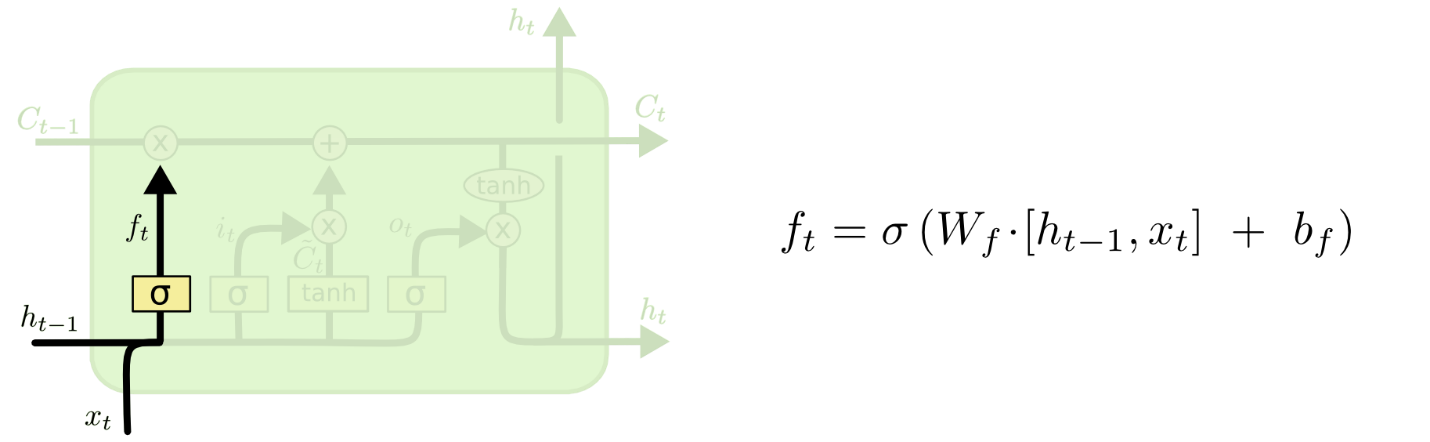
\includegraphics[width=15cm]{chaps/lr/lstm_3}}
	\caption{
		قدم اول در پاک کردن اطلاعات از سلول حالت در وضعیت ورودی
	}
	\label{fig:ch_lr:lstm_3}
\end{figure} 
\\
قدم بعدی این است که تصمیم بگیریم چه اطلاعات جدیدی را می‌خواهیم در سلول حالت ذخیره کنیم. این تصمیم دو بخشی است. ابتدا یک لایه سیگموید به نام دروازه ورودی\LTRfootnote{Input gate} داریم که تصمیم می‌گیرد چه مقادیری به‌روز خواهند شد. مرحله بعدی یک لایه تانژانت هایپربولیک است که برداری از مقادیر به نام $\tilde{C}_t$ می‌سازد که می‌توان آن‌ها را به سلول حالت اضافه کرد. در مرحله بعد، ما این دو مرحله را با هم ترکیب می‌کنیم تا مقدار سلول حالت را به‌روز کنیم.
\\
در مثال مدل زبانی‌ای که پیش‌تر داشتیم، قصد داریم جنسیت فاعل جدید را به سلول حالت اضافه کنیم تا جایگزین جنسیت فاعل قبلی شود که در مرحله قبلی تصمیم گرفتیم آن را فراموش کنیم.
 \begin{figure}[!ht]
	\centerline{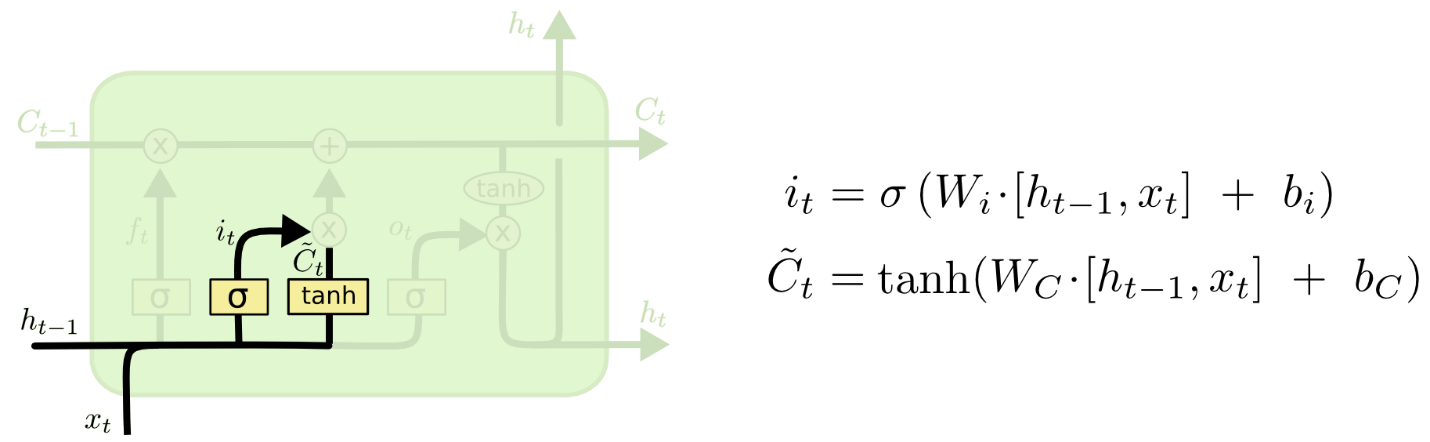
\includegraphics[width=15cm]{chaps/lr/lstm_4}}
	\caption{
		قدم دوم در اضافه کردن اطلاعات جدید به سلول حالت
	}
	\label{fig:ch_lr:lstm_4}
\end{figure} 
\\
حال زمان آن فرا رسیده است که سلول حالت قدیمی یعنی $C_{t-1}$ را سلول حالت جدید یعنی $C_t$ به‌روز کنیم. در مراحل قبلی تصمیم گرفته شد که چه کنیم و در حال حاضر تنها لازم است تصمیماتی را که گرفته شد عملی کنیم.
\\
ما مقدار قبلی سلول حالت را در $f_t$ ضرب می‌کنیم که یعنی فراموش کردن اطلاعاتی که پیش‌تر تصمیم گرفتیم آن‌ها را فراموش کنیم. سپس $i_t \ast \tilde{C}_t$ را به آن اضافه می‌کنیم. در حال حاضر مقادیر جدید سلول حالت با توجه به تصمیماتی که پیش‌تر گرفته شده بود بدست آمده‌اند. در مثال مدل زبانی، اینجا دقیقاً جائی است که اطلاعاتی که در مورد جنسیت قبلی داشتیم را دور می‌ریزیم و اطلاعات جدید را اضافه می‌کنیم.
 \begin{figure}[!ht]
	\centerline{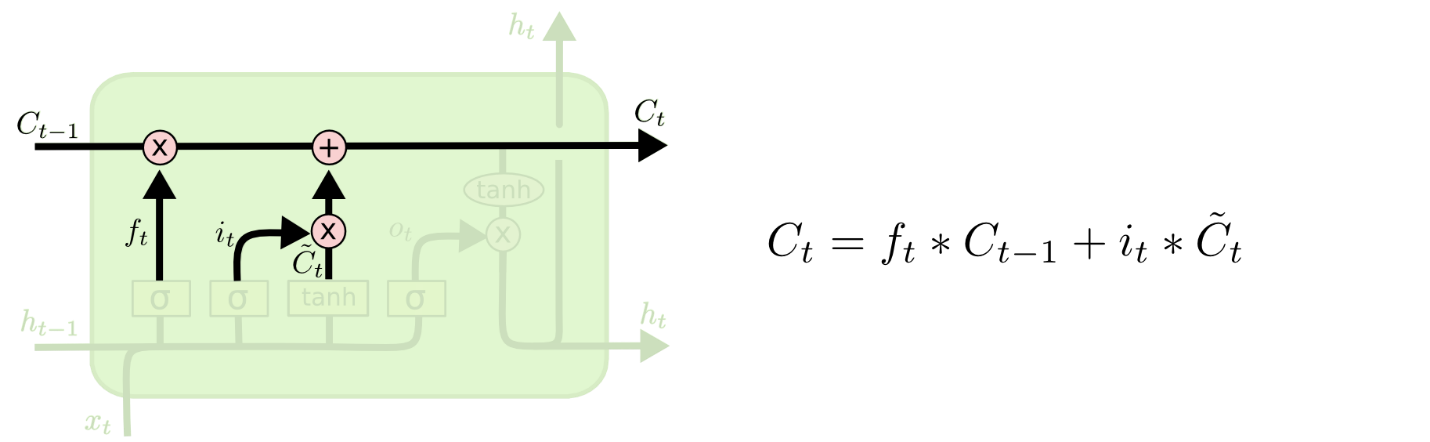
\includegraphics[width=15cm]{chaps/lr/lstm_5}}
	\caption{
		به‌روز رسانی اطلاعات در سلول حالت
	}
	\label{fig:ch_lr:lstm_5}
\end{figure} 
\\
در نهایت باید تصمیم بگیریم قرار است چه اطلاعاتی را به خروجی ببریم. این خروجی با در نظر گرفتن مقدار سلول حالت خواهد بود، ولی از فیلتر مشخصی عبور خواهد کرد. در ابتدا، یک لایه سیگموید داریم که تصمیم می‌گیرد چه بخشی از سلول حالت قرار است به خروجی برده شود. سپس مقدار سلول حالت (پس از به‌روز شدن در مراحل قبلی) را به یک لایه تانژانت هایپربولیک (تا مقادیر بین $-1$ و $+1$ باشند) می‌دهیم و مقدار آن را در خروجی لایه \gls{sigmoid} قبلی ضرب می‌کنیم تا تنها بخش‌هایی که مد نظرمان است به خروجی برود.
\\
در مثال مدل زبانی، با توجه به اینکه تنها فاعل را دیده‌است، در صورتی که بخواهیم کلمه بعدی را حدس بزنیم، ممکن است بخواهد اطلاعاتی در ارتباط با فعل را به خروجی ببرد. برای مثال ممکن است اینکه فاعل مفرد یا جمع است را به خروجی ببرد، که ما با توجه به آن بدانیم فعل به چه فرمی خواهد بود.
 \begin{figure}[!ht]
	\centerline{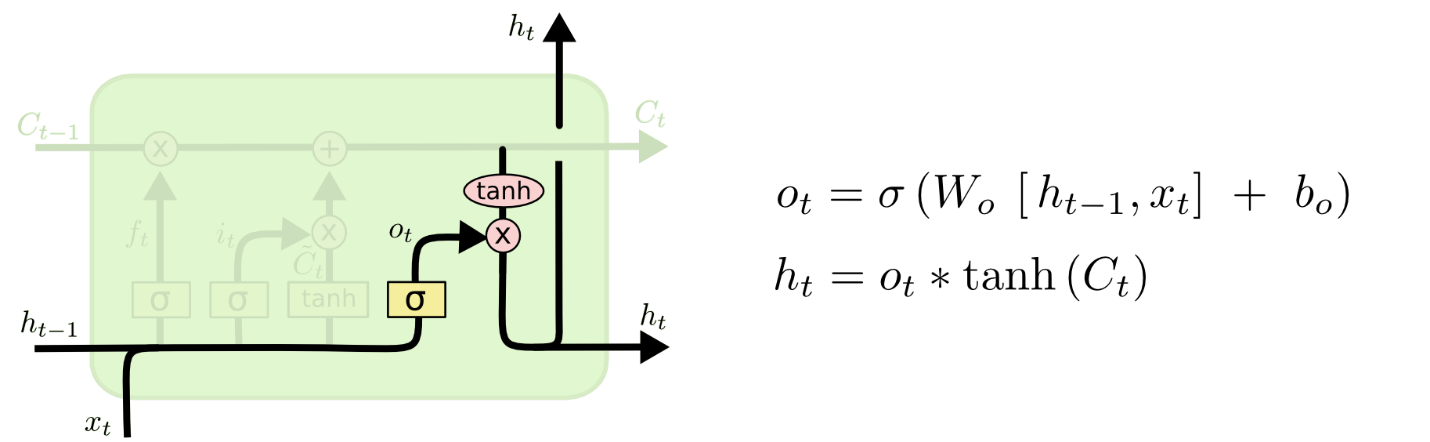
\includegraphics[width=15cm]{chaps/lr/lstm_6}}
	\caption{
		قدم نهایی برای تولید خروجی ماژول \lr{LSTM}
	}
	\label{fig:ch_lr:lstm_6}
\end{figure} 
 
 \section{\gls{reinforcementlearning}}
 
 \subsection{مقدمه و بیشینه تاریخی}
 ادوارد ثورندایک\LTRfootnote{Edward Thorndike} پدر روانشناسی مدرن در سال 1874 میلادی در ایالت ماساچوست آمریکا متولد شد. وی در اوایل قرن 20 میلادی آزمایشی انجام داد که باعث ارائه قانون اثر شد. او برای این آزمایش، گربه ای را در جعبه ای موسوم به جعبه معما قرار داد. هر کوشش درستی، از این گربه برای نجات از جعبه صورت می‌گرفت، باعث میشد ثورندایک به عنوان پاداش به او غذا بدهد. به تدریج گربه به کارهای درست خود پی برد و آنها را تکرار کرد، تا جایی که دیگر هیچ کار اشتباهی نمی کرد و بلاخره موفق به خروج از جعبه شد. ثورندایک در سال 1912 به ریاست انجمن روانشناسان، در سال 1917 به عضویت انجمن علوم، در سال 1934به ریاست انجمن علوم پیشرفته نایل آمد و در سال 1947 در سن 74 سالگی، بدرود حیات گفت. در سال 2002 رتبه ای از برترین روانشناسان تاریخ ارائه شد که ثورندایک جزء 10 روانشناس برتر تاریخ قرار گرفت. می‌توان مهم ترین کشف وی را، اثبات وجود یادگیری تقویتی در روانشناسی دانست.
 
 شاید ریچارد بلمن\LTRfootnote{Richard E. Bellman} (مخترع الگوریتم بلمن-فورد) را بتوان اولین کسی دانست که یادگیری تقویتی را وارد هوش مصنوعی ساخت. در اوایل دهه 1950 بلمن مسئله ای با عنوان «کنترل بهینه» را مطرح ساخت که با استفاده از روش های پویا در برنامه ریزی پویا کنترل کننده ها را به سمت نتیجه بهینه رهنمون می‌شد. در اواخر دهه 50 میلادی مینسکی در پایان نامه دکتری خود روش های محاسبات آزمون و خطا توسط مفهوم یادگیری تقویتی را مطرح نمود و الگوریتم های یادگیری تقویتی را پایه ریزی کرد. در کل دهه 50 میلادی را میتوان دهه تشکیل الگوریتم های محاسباتی اولیه یادگیری تقویتی دانست. در دهه 60 میلادی اولین کابرد های یادگیری تقویتی به وقوع پیوستند. در اولین تلاش ها فارلی و کلارک از یادگیری تقویتی برای تشخیص الگو استفاده کردند بدین صورت که هر بار برنامه نتیجه بهتری به دست می‌آمد او را تشویق می‌کردند. در اواخر دهه 60 میلادی، یادگیری نظارتی از یادگیری تقویتی ، مشتق شد. در یادگیری نظارتی طراح نتیجه نهایی را در دست دارد و از هوش مصنوعی می‌خواهد هر بار مسیر بین ورودی و نتیجه را طراحی کرده و هربار که برنامه، مسیر بهتری به دست می‌آورد، تشویق می‌شود. همچنین طراح نظارت مستقیم بر عملکرد عامل دارد.



 